% Options for packages loaded elsewhere
\PassOptionsToPackage{unicode}{hyperref}
\PassOptionsToPackage{hyphens}{url}
%
\documentclass[
  9 pt,
  ignorenonframetext,
]{beamer}
\usepackage{pgfpages}
\setbeamertemplate{caption}[numbered]
\setbeamertemplate{caption label separator}{: }
\setbeamercolor{caption name}{fg=normal text.fg}
\beamertemplatenavigationsymbolsempty
% Prevent slide breaks in the middle of a paragraph
\widowpenalties 1 10000
\raggedbottom
\setbeamertemplate{part page}{
  \centering
  \begin{beamercolorbox}[sep=16pt,center]{part title}
    \usebeamerfont{part title}\insertpart\par
  \end{beamercolorbox}
}
\setbeamertemplate{section page}{
  \centering
  \begin{beamercolorbox}[sep=12pt,center]{part title}
    \usebeamerfont{section title}\insertsection\par
  \end{beamercolorbox}
}
\setbeamertemplate{subsection page}{
  \centering
  \begin{beamercolorbox}[sep=8pt,center]{part title}
    \usebeamerfont{subsection title}\insertsubsection\par
  \end{beamercolorbox}
}
\AtBeginPart{
  \frame{\partpage}
}
\AtBeginSection{
  \ifbibliography
  \else
    \frame{\sectionpage}
  \fi
}
\AtBeginSubsection{
  \frame{\subsectionpage}
}
\usepackage{amsmath,amssymb}
\usepackage{lmodern}
\usepackage{ifxetex,ifluatex}
\ifnum 0\ifxetex 1\fi\ifluatex 1\fi=0 % if pdftex
  \usepackage[T1]{fontenc}
  \usepackage[utf8]{inputenc}
  \usepackage{textcomp} % provide euro and other symbols
\else % if luatex or xetex
  \usepackage{unicode-math}
  \defaultfontfeatures{Scale=MatchLowercase}
  \defaultfontfeatures[\rmfamily]{Ligatures=TeX,Scale=1}
\fi
\usetheme[]{Dresden}
\usecolortheme{seagull}
\usefonttheme{structuresmallcapsserif}
% Use upquote if available, for straight quotes in verbatim environments
\IfFileExists{upquote.sty}{\usepackage{upquote}}{}
\IfFileExists{microtype.sty}{% use microtype if available
  \usepackage[]{microtype}
  \UseMicrotypeSet[protrusion]{basicmath} % disable protrusion for tt fonts
}{}
\makeatletter
\@ifundefined{KOMAClassName}{% if non-KOMA class
  \IfFileExists{parskip.sty}{%
    \usepackage{parskip}
  }{% else
    \setlength{\parindent}{0pt}
    \setlength{\parskip}{6pt plus 2pt minus 1pt}}
}{% if KOMA class
  \KOMAoptions{parskip=half}}
\makeatother
\usepackage{xcolor}
\IfFileExists{xurl.sty}{\usepackage{xurl}}{} % add URL line breaks if available
\IfFileExists{bookmark.sty}{\usepackage{bookmark}}{\usepackage{hyperref}}
\hypersetup{
  pdftitle={Modelagem XGBOOST para a classificação de avaliações de livros},
  pdfauthor={Ana Luzielma Campos ; Jaylhane Nunes ; Raianny Soares},
  hidelinks,
  pdfcreator={LaTeX via pandoc}}
\urlstyle{same} % disable monospaced font for URLs
\newif\ifbibliography
\usepackage{color}
\usepackage{fancyvrb}
\newcommand{\VerbBar}{|}
\newcommand{\VERB}{\Verb[commandchars=\\\{\}]}
\DefineVerbatimEnvironment{Highlighting}{Verbatim}{commandchars=\\\{\}}
% Add ',fontsize=\small' for more characters per line
\usepackage{framed}
\definecolor{shadecolor}{RGB}{248,248,248}
\newenvironment{Shaded}{\begin{snugshade}}{\end{snugshade}}
\newcommand{\AlertTok}[1]{\textcolor[rgb]{0.94,0.16,0.16}{#1}}
\newcommand{\AnnotationTok}[1]{\textcolor[rgb]{0.56,0.35,0.01}{\textbf{\textit{#1}}}}
\newcommand{\AttributeTok}[1]{\textcolor[rgb]{0.77,0.63,0.00}{#1}}
\newcommand{\BaseNTok}[1]{\textcolor[rgb]{0.00,0.00,0.81}{#1}}
\newcommand{\BuiltInTok}[1]{#1}
\newcommand{\CharTok}[1]{\textcolor[rgb]{0.31,0.60,0.02}{#1}}
\newcommand{\CommentTok}[1]{\textcolor[rgb]{0.56,0.35,0.01}{\textit{#1}}}
\newcommand{\CommentVarTok}[1]{\textcolor[rgb]{0.56,0.35,0.01}{\textbf{\textit{#1}}}}
\newcommand{\ConstantTok}[1]{\textcolor[rgb]{0.00,0.00,0.00}{#1}}
\newcommand{\ControlFlowTok}[1]{\textcolor[rgb]{0.13,0.29,0.53}{\textbf{#1}}}
\newcommand{\DataTypeTok}[1]{\textcolor[rgb]{0.13,0.29,0.53}{#1}}
\newcommand{\DecValTok}[1]{\textcolor[rgb]{0.00,0.00,0.81}{#1}}
\newcommand{\DocumentationTok}[1]{\textcolor[rgb]{0.56,0.35,0.01}{\textbf{\textit{#1}}}}
\newcommand{\ErrorTok}[1]{\textcolor[rgb]{0.64,0.00,0.00}{\textbf{#1}}}
\newcommand{\ExtensionTok}[1]{#1}
\newcommand{\FloatTok}[1]{\textcolor[rgb]{0.00,0.00,0.81}{#1}}
\newcommand{\FunctionTok}[1]{\textcolor[rgb]{0.00,0.00,0.00}{#1}}
\newcommand{\ImportTok}[1]{#1}
\newcommand{\InformationTok}[1]{\textcolor[rgb]{0.56,0.35,0.01}{\textbf{\textit{#1}}}}
\newcommand{\KeywordTok}[1]{\textcolor[rgb]{0.13,0.29,0.53}{\textbf{#1}}}
\newcommand{\NormalTok}[1]{#1}
\newcommand{\OperatorTok}[1]{\textcolor[rgb]{0.81,0.36,0.00}{\textbf{#1}}}
\newcommand{\OtherTok}[1]{\textcolor[rgb]{0.56,0.35,0.01}{#1}}
\newcommand{\PreprocessorTok}[1]{\textcolor[rgb]{0.56,0.35,0.01}{\textit{#1}}}
\newcommand{\RegionMarkerTok}[1]{#1}
\newcommand{\SpecialCharTok}[1]{\textcolor[rgb]{0.00,0.00,0.00}{#1}}
\newcommand{\SpecialStringTok}[1]{\textcolor[rgb]{0.31,0.60,0.02}{#1}}
\newcommand{\StringTok}[1]{\textcolor[rgb]{0.31,0.60,0.02}{#1}}
\newcommand{\VariableTok}[1]{\textcolor[rgb]{0.00,0.00,0.00}{#1}}
\newcommand{\VerbatimStringTok}[1]{\textcolor[rgb]{0.31,0.60,0.02}{#1}}
\newcommand{\WarningTok}[1]{\textcolor[rgb]{0.56,0.35,0.01}{\textbf{\textit{#1}}}}
\usepackage{graphicx}
\makeatletter
\def\maxwidth{\ifdim\Gin@nat@width>\linewidth\linewidth\else\Gin@nat@width\fi}
\def\maxheight{\ifdim\Gin@nat@height>\textheight\textheight\else\Gin@nat@height\fi}
\makeatother
% Scale images if necessary, so that they will not overflow the page
% margins by default, and it is still possible to overwrite the defaults
% using explicit options in \includegraphics[width, height, ...]{}
\setkeys{Gin}{width=\maxwidth,height=\maxheight,keepaspectratio}
% Set default figure placement to htbp
\makeatletter
\def\fps@figure{htbp}
\makeatother
\setlength{\emergencystretch}{3em} % prevent overfull lines
\providecommand{\tightlist}{%
  \setlength{\itemsep}{0pt}\setlength{\parskip}{0pt}}
\setcounter{secnumdepth}{-\maxdimen} % remove section numbering
\usepackage[brazilian]{babel}
\usepackage{float}
\floatplacement{figure}{H}
\usepackage[utf8]{inputenc}
\usepackage{pagecolor}
\usepackage{xcolor}
\usepackage{indentfirst}
\setlength\parindent{22pt}
\usepackage{longtable,booktabs}
\ifluatex
  \usepackage{selnolig}  % disable illegal ligatures
\fi

\title{Modelagem XGBOOST para a classificação de avaliações de livros}
\author{Ana Luzielma Campos \newline \and Jaylhane Nunes
\newline \and Raianny Soares}
\date{07/02/2022}

\begin{document}
\frame{\titlepage}

\hypertarget{introduuxe7uxe3o}{%
\section{Introdução}\label{introduuxe7uxe3o}}

\hypertarget{contextualizauxe7uxe3o}{%
\subsubsection{Contextualização}\label{contextualizauxe7uxe3o}}

\begin{frame}{Contextualização}
Motivadas pelo interesse comum em leitura optamos por realizar a análise
de um conjuntos de dados envolvendo livros.

O conjunto de dados selecionado possui \textbf{11.131 observações}, foi
gerado por meio de \textbf{raspagem} de dados na \textbf{API} da
plataforma \textbf{GoodReads} e disponibilizado por
\textbf{\emph{Soumik}} no site \textbf{Kagle}.

Nele é possível encontrar as 12 colunas seguintes:

\begin{table}[H]
\centering
\begin{tabular}{llll}
\toprule
bookID & average\_rating & language\_code & text\_reviews\_count\\
title & isbn & num\_pages & publication\_date\\
authors & isbn13 & ratings\_count & publisher\\
\bottomrule
\end{tabular}
\end{table}

Chegamos a um consenso que diversos fatores influenciam na satisfação
com a leitura e quisemos investigar se, com os dados disponíveis, seria
possível obter um modelo que conseguisse predizer se o livro foi
considerado: \emph{ruim}, \emph{bom} ou \emph{ótimo} .
\end{frame}

\hypertarget{uma-ideia-inicial}{%
\subsubsection{Uma Ideia Inicial}\label{uma-ideia-inicial}}

\begin{frame}{Uma Ideia Inicial}
\begin{figure}
\centering
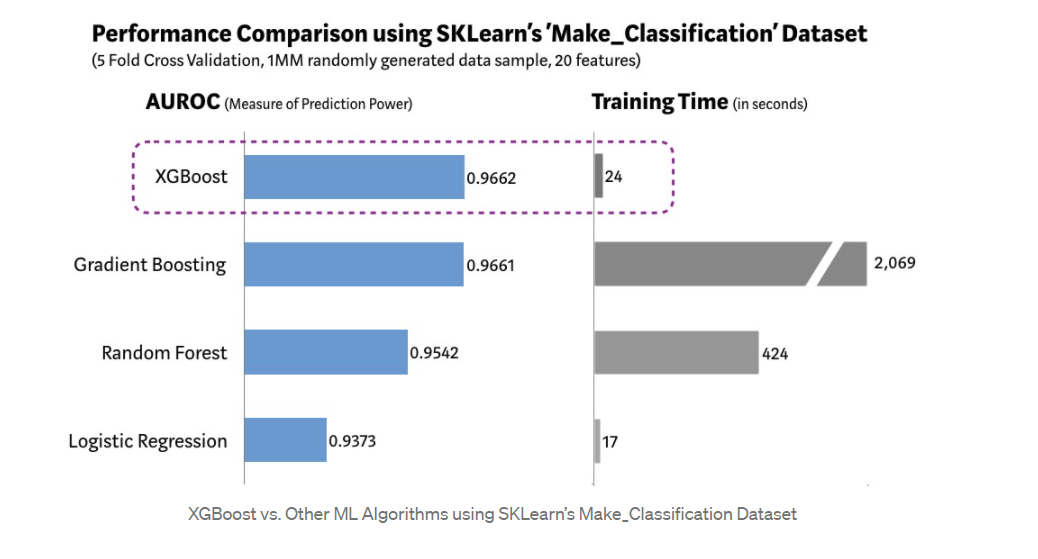
\includegraphics[width=0.75\textwidth,height=\textheight]{./Imagens/desempenho_xgboost_comparacao.png}
\caption{Vishal Morde, 2019 - XGBoost Algorithm: Long May She Reign!}
\end{figure}

Dentre as possibilidades percebemos que o \textbf{XGboost} tem um ótimo
desempenho comparado a outros e que, apesar da nossa variável de
avaliação ser uma variável contínua, um método de classificação poderia
ser adequado, desde que encaixássemos intervalos em categorias.
\end{frame}

\hypertarget{a-inspirauxe7uxe3o-final}{%
\subsubsection{A Inspiração Final}\label{a-inspirauxe7uxe3o-final}}

\begin{frame}{A Inspiração Final}
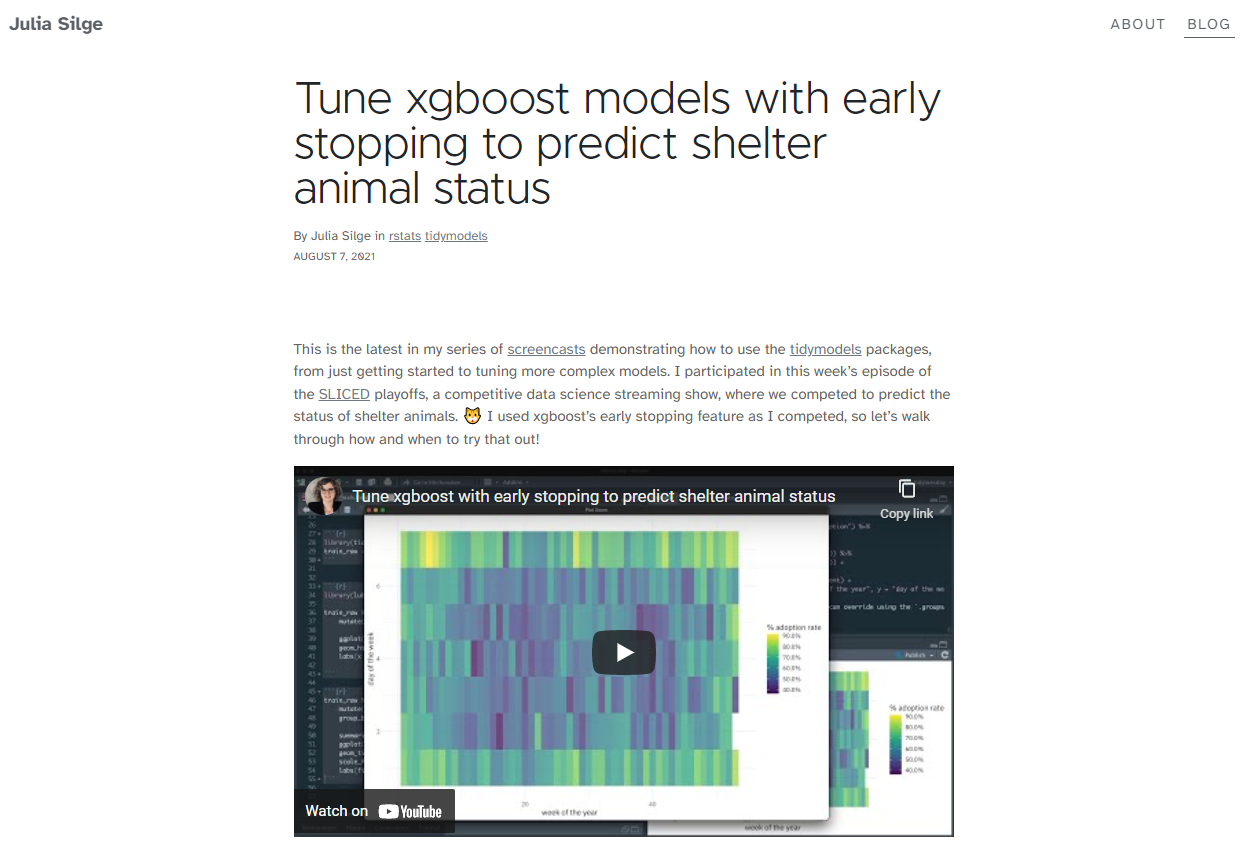
\includegraphics[width=\textwidth,height=0.9\textheight]{./Imagens/xgboost_juliasilge.png}
\end{frame}

\hypertarget{indicamos}{%
\subsubsection{Indicamos}\label{indicamos}}

\begin{frame}{Indicamos}

\includegraphics{./Imagens/juliasilge_mini.png} juliasilge.com

\begin{itemize}
\tightlist
\item
  \emph{Agora, à nossa análise!}
\end{itemize}
\end{frame}

\hypertarget{desenvolvimento}{%
\section{Desenvolvimento}\label{desenvolvimento}}

\hypertarget{engenharia-de-dados}{%
\subsubsection{Engenharia de Dados}\label{engenharia-de-dados}}

\begin{frame}{Engenharia de Dados}
A análise exploratória consistiu em:

\begin{itemize}
\tightlist
\item
  Limpeza dos Dados
\item
  Análise Descritiva
\end{itemize}

Dado os nossos objetivos percebemos que algumas colunas eram
dispensáveis e outras poderiam ser transformadas, de forma que:

\begin{table}[H]
\centering
\begin{tabular}{lll}
\toprule
Excluídas & Transfomadas & Geradas\\
\midrule
bookID & average\_rating & book\_rating¹\\
title & language\_code & \\
isbn & text\_reviews\_count & prop\_text\_reviews²\\
authors & publication\_date & book\_age\\
isbn13 &  & \\
\addlinespace
publisher &  & \\
\bottomrule
\end{tabular}
\end{table}

\begin{block}{\emph{Nosso \textbf{MAIOR} desafio durante a análise e a
modelagem esteve relacionado a essa fase de engenharia de dados}}
\protect\hypertarget{nosso-maior-desafio-durante-a-anuxe1lise-e-a-modelagem-esteve-relacionado-a-essa-fase-de-engenharia-de-dados}{}
\end{block}
\end{frame}

\hypertarget{anuxe1lise-exploratuxf3ria}{%
\subsubsection{Análise Exploratória}\label{anuxe1lise-exploratuxf3ria}}

\begin{frame}[fragile]{Análise Exploratória}
\begin{itemize}
\tightlist
\item
  Para iniciar separamos o conjunto em \textbf{treino} e \textbf{teste}
  baseando-nos em 75\% das observações e balanceando-as com nossa
  variável resposta: \texttt{book\_rating}.
\end{itemize}

\begin{Shaded}
\begin{Highlighting}[]
\FunctionTok{set.seed}\NormalTok{(}\DecValTok{1904}\NormalTok{, }\AttributeTok{kind =} \StringTok{"Mersenne{-}Twister"}\NormalTok{, }\AttributeTok{normal.kind =} \StringTok{"Inversion"}\NormalTok{)}
\NormalTok{livros\_split }\OtherTok{\textless{}{-}} \FunctionTok{initial\_split}\NormalTok{(livros, }\AttributeTok{prop =}\NormalTok{ .}\DecValTok{75}\NormalTok{, }\AttributeTok{strata =}\NormalTok{ book\_rating)}
\NormalTok{livros\_treino }\OtherTok{\textless{}{-}} \FunctionTok{training}\NormalTok{(livros\_split)}
\NormalTok{livros\_teste }\OtherTok{\textless{}{-}} \FunctionTok{testing}\NormalTok{(livros\_split)}
\end{Highlighting}
\end{Shaded}

\begin{itemize}
\tightlist
\item
  Em seguida verificamos a dispersão e correlação entre as variáveis
  numéricas:
\end{itemize}

\begin{Shaded}
\begin{Highlighting}[]
\NormalTok{livros\_treino }\SpecialCharTok{\%\textgreater{}\%} 
  \FunctionTok{select}\NormalTok{(}\FunctionTok{where}\NormalTok{(is.numeric)) }\SpecialCharTok{\%\textgreater{}\%} 
  \FunctionTok{ggpairs}\NormalTok{(}\AttributeTok{upper =} \FunctionTok{list}\NormalTok{(}\AttributeTok{continuous =} \FunctionTok{wrap}\NormalTok{(}\StringTok{"cor"}\NormalTok{, }\AttributeTok{method =} \StringTok{"spearman"}\NormalTok{)))}
\end{Highlighting}
\end{Shaded}
\end{frame}

\hypertarget{anuxe1lise-exploratuxf3ria-1}{%
\subsubsection{Análise
Exploratória}\label{anuxe1lise-exploratuxf3ria-1}}

\begin{frame}{Análise Exploratória}
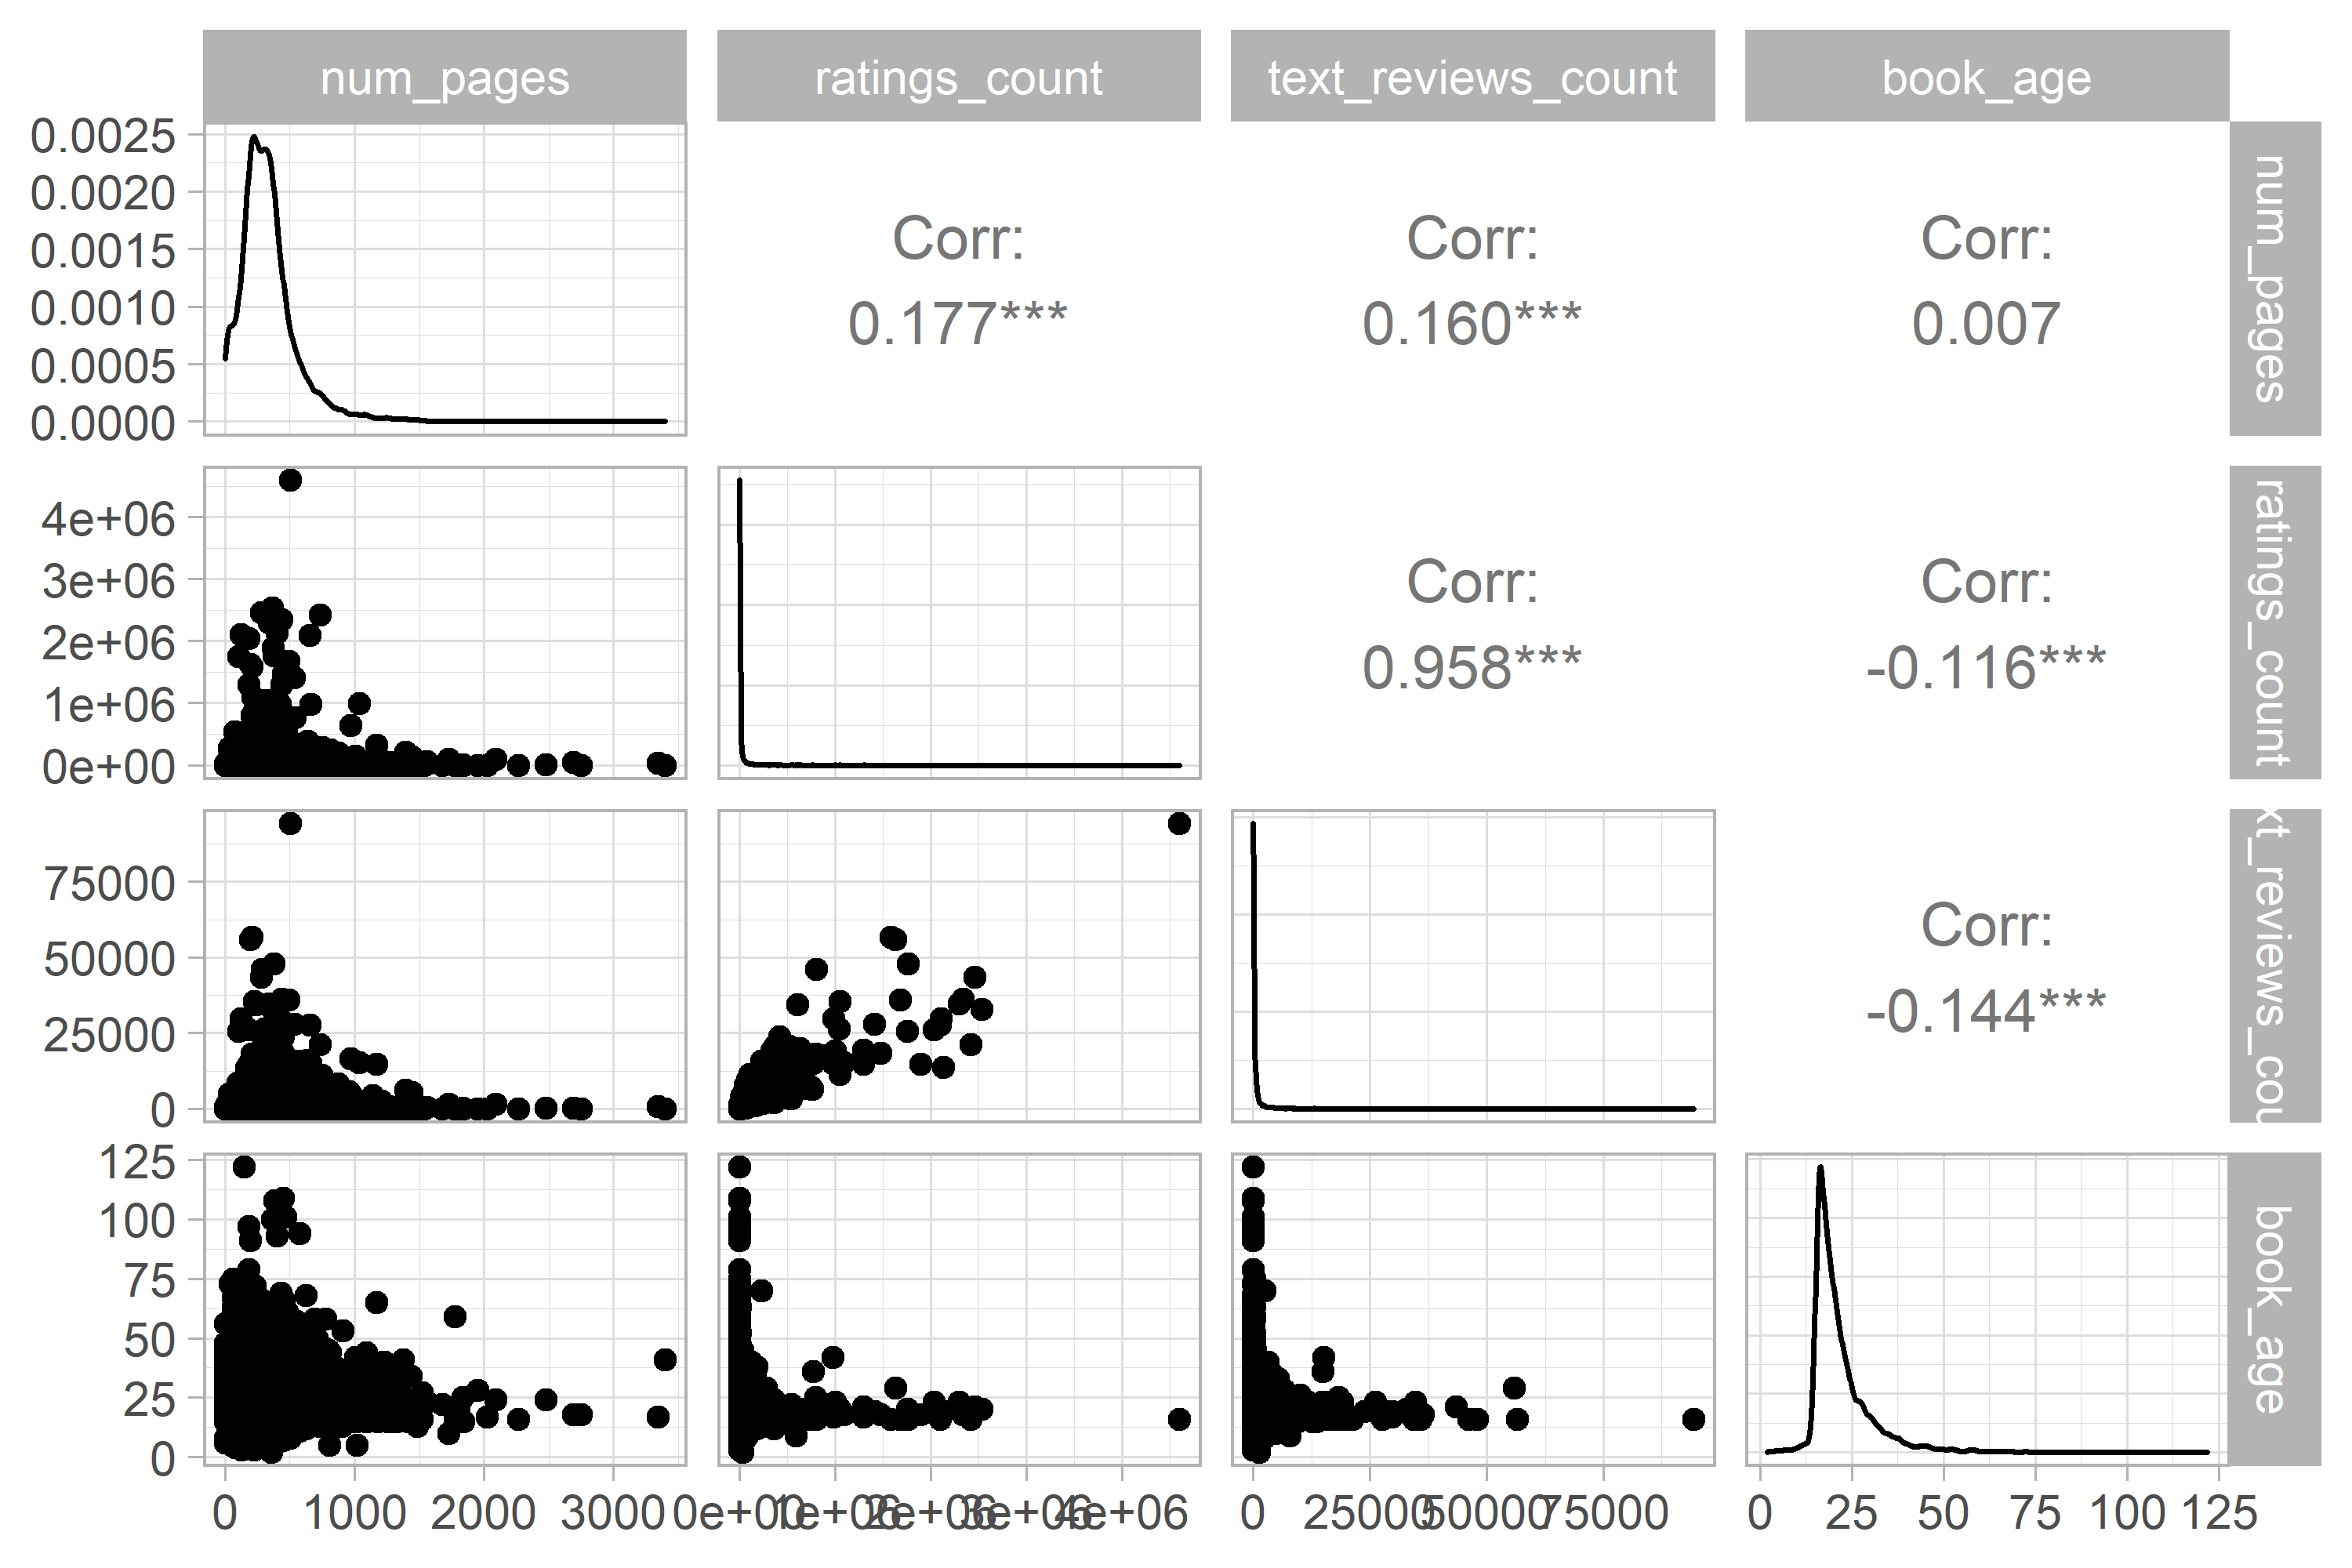
\includegraphics{apresentacao_files/figure-beamer/unnamed-chunk-5-1.png}
\end{frame}

\hypertarget{anuxe1lise-exploratuxf3ria-2}{%
\subsubsection{Análise
Exploratória}\label{anuxe1lise-exploratuxf3ria-2}}

\begin{frame}[fragile]{Análise Exploratória}
Com o resultado anterior percebemos que:

\begin{itemize}
\tightlist
\item
  Correlação forte entre \texttt{text\_reviews\_count} e
  \texttt{ratings\_count}.
\item
  Seria necessário descartar \texttt{text\_reviews\_count} devido riscos
  de multicolineariedade, mas como consideramos as avaliações escritas
  relevantes para as categorias \emph{ruim} e \emph{ótimo} usamos a
  proporção entre \texttt{text\_reviews\_count}/\texttt{ratings\_count}.
\end{itemize}

\begin{Shaded}
\begin{Highlighting}[]
\NormalTok{livros\_treino }\OtherTok{\textless{}{-}}\NormalTok{ livros\_treino }\SpecialCharTok{\%\textgreater{}\%} 
  \FunctionTok{mutate}\NormalTok{(}\AttributeTok{prop\_text\_reviews =}\NormalTok{ text\_reviews\_count }\SpecialCharTok{/}\NormalTok{ ratings\_count) }\SpecialCharTok{\%\textgreater{}\%} 
  \FunctionTok{select}\NormalTok{(}\SpecialCharTok{{-}}\NormalTok{text\_reviews\_count)}

\FunctionTok{cor}\NormalTok{(livros\_treino}\SpecialCharTok{$}\NormalTok{prop\_text\_reviews,livros\_treino}\SpecialCharTok{$}\NormalTok{ratings\_count,}
    \AttributeTok{use =} \StringTok{"complete"}\NormalTok{, }\AttributeTok{method =} \StringTok{"spearman"}\NormalTok{)}
\end{Highlighting}
\end{Shaded}

{[}1{]} -0.3605

\begin{itemize}
\tightlist
\item
  A correlação entre \texttt{prop\_text\_reviews} e
  \texttt{ratings\_count} não indicou multicolinearidade, então
  prosseguimos com essa variável como preditora.
\end{itemize}
\end{frame}

\hypertarget{continuando-a-anuxe1lise-exploratuxf3ria-e-descritiva}{%
\subsubsection{Continuando a Análise Exploratória e
Descritiva}\label{continuando-a-anuxe1lise-exploratuxf3ria-e-descritiva}}

\begin{frame}{Continuando a Análise Exploratória e Descritiva}
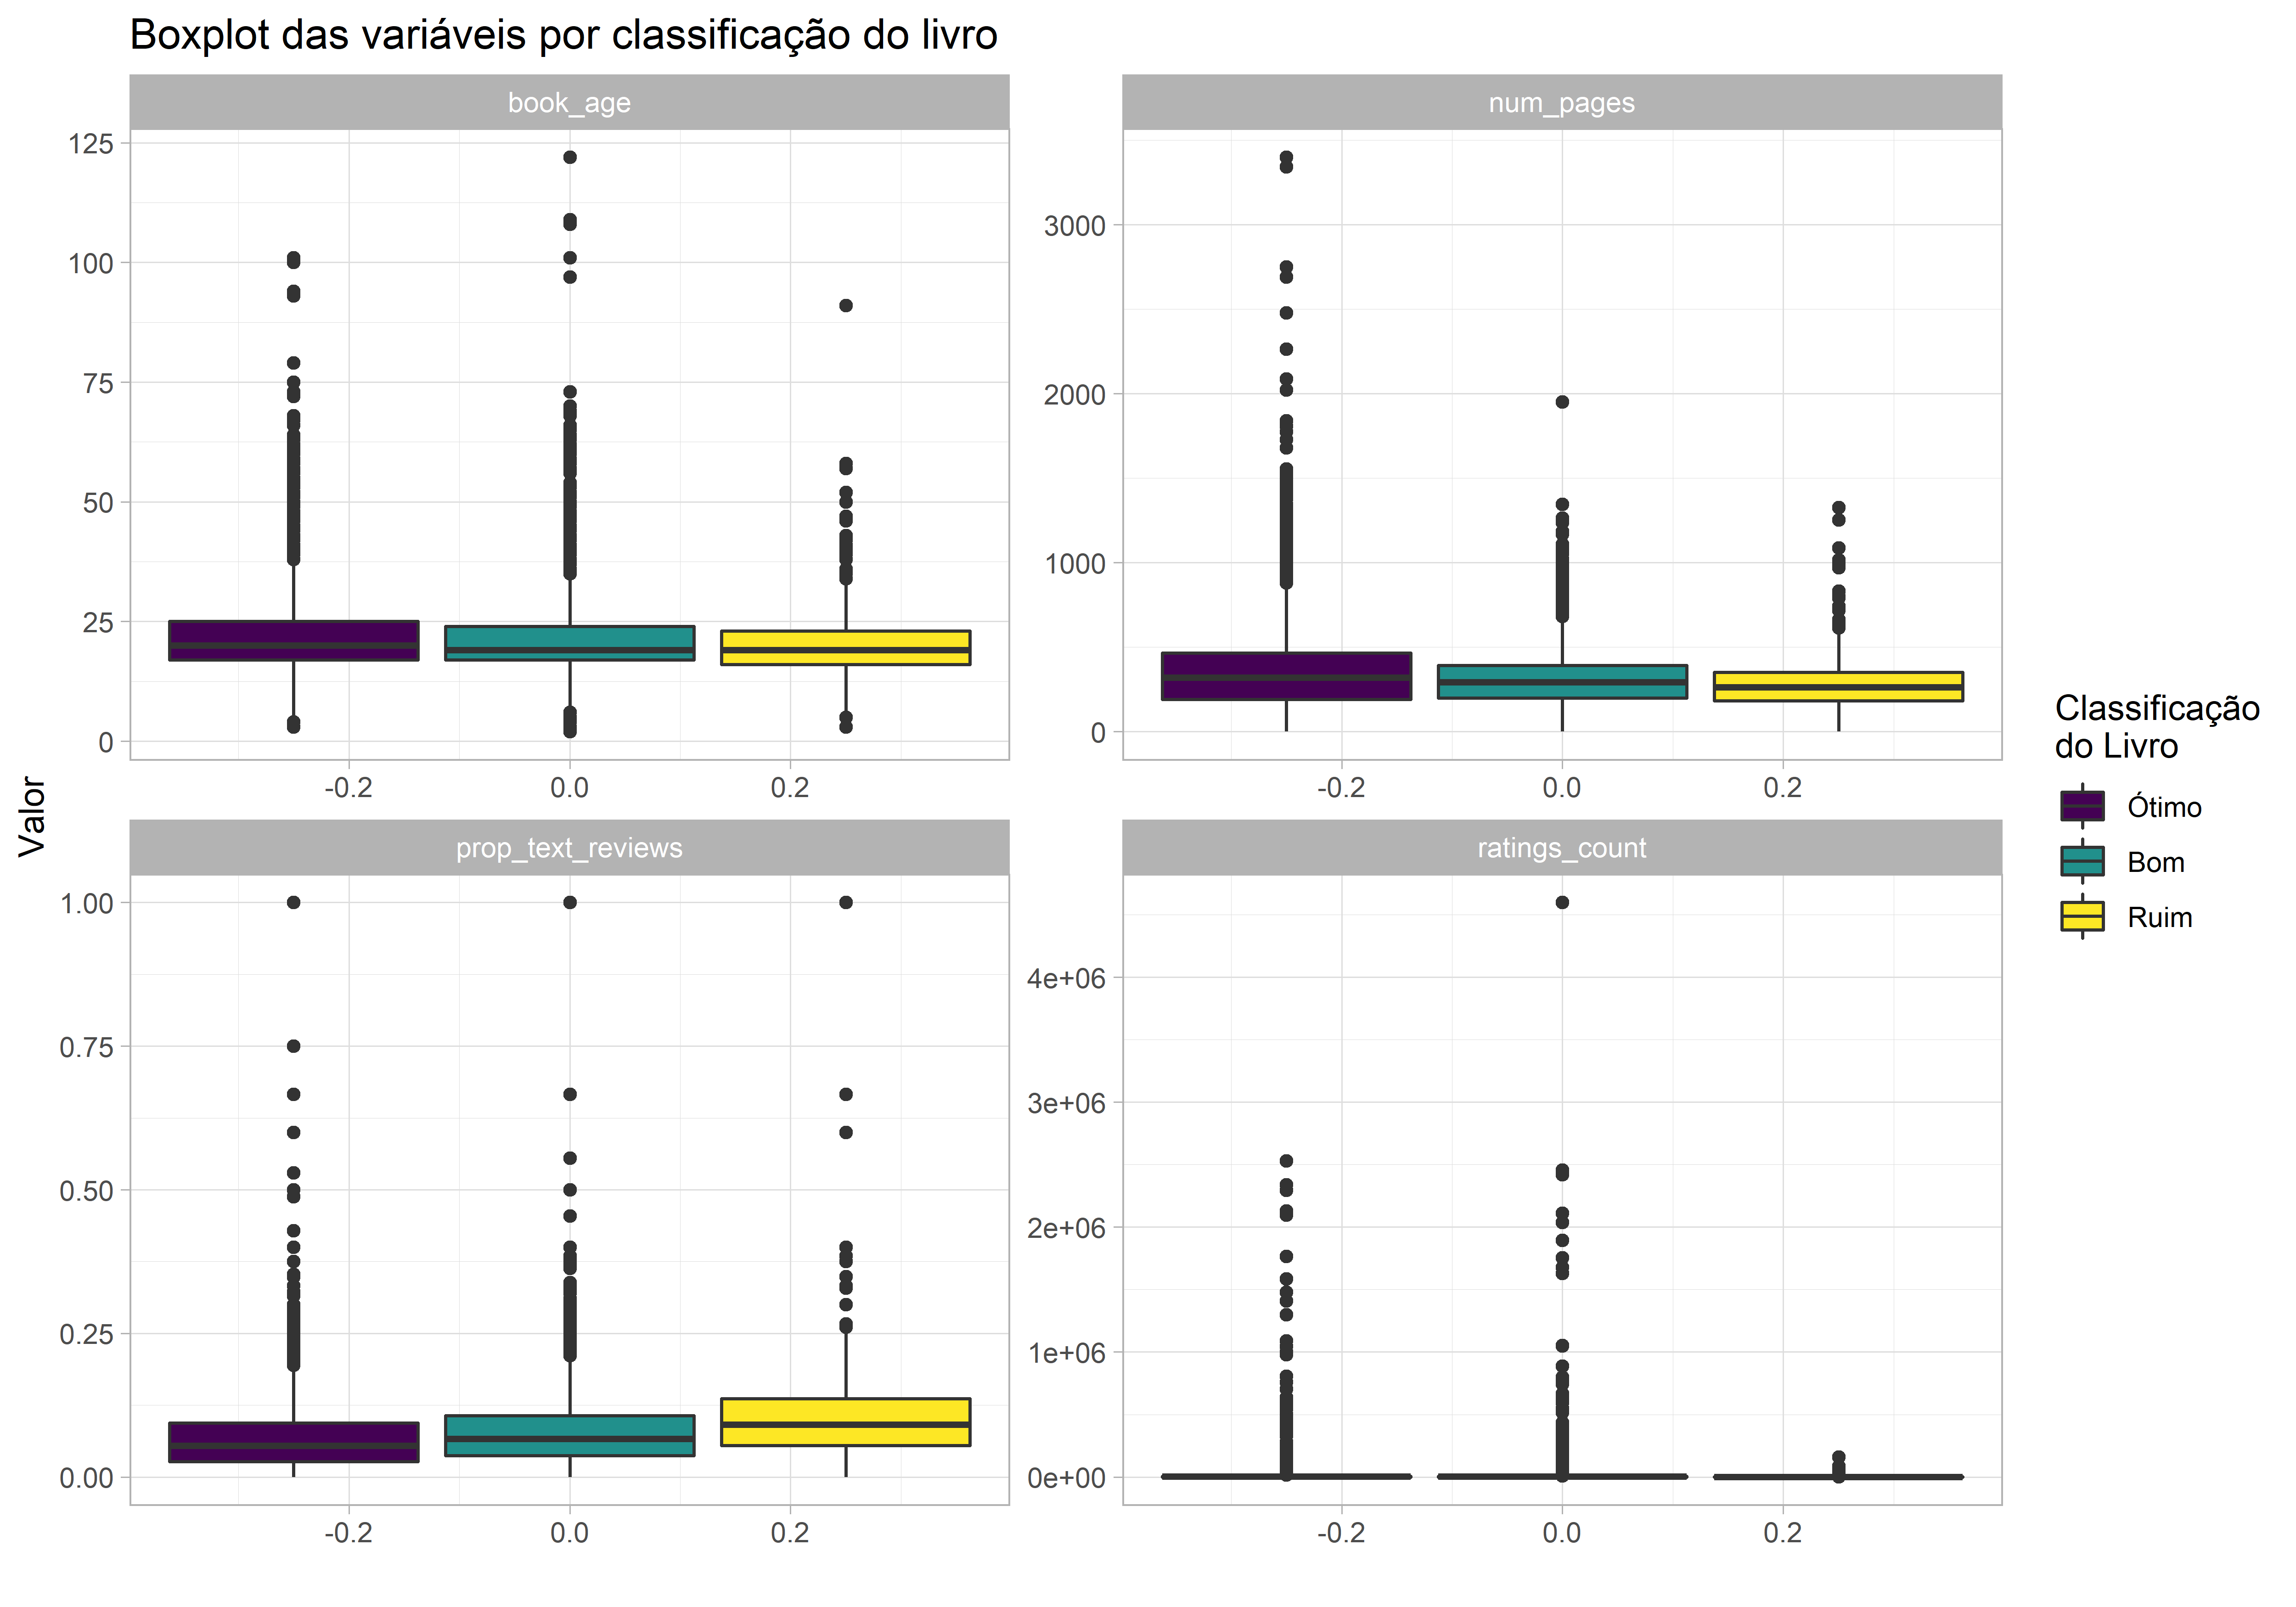
\includegraphics{apresentacao_files/figure-beamer/unnamed-chunk-7-1.png}
\end{frame}

\hypertarget{conferindo-aspectos-que-consideramos-importantes}{%
\subsubsection{Conferindo aspectos que consideramos
importantes}\label{conferindo-aspectos-que-consideramos-importantes}}

\begin{frame}{Conferindo aspectos que consideramos importantes}
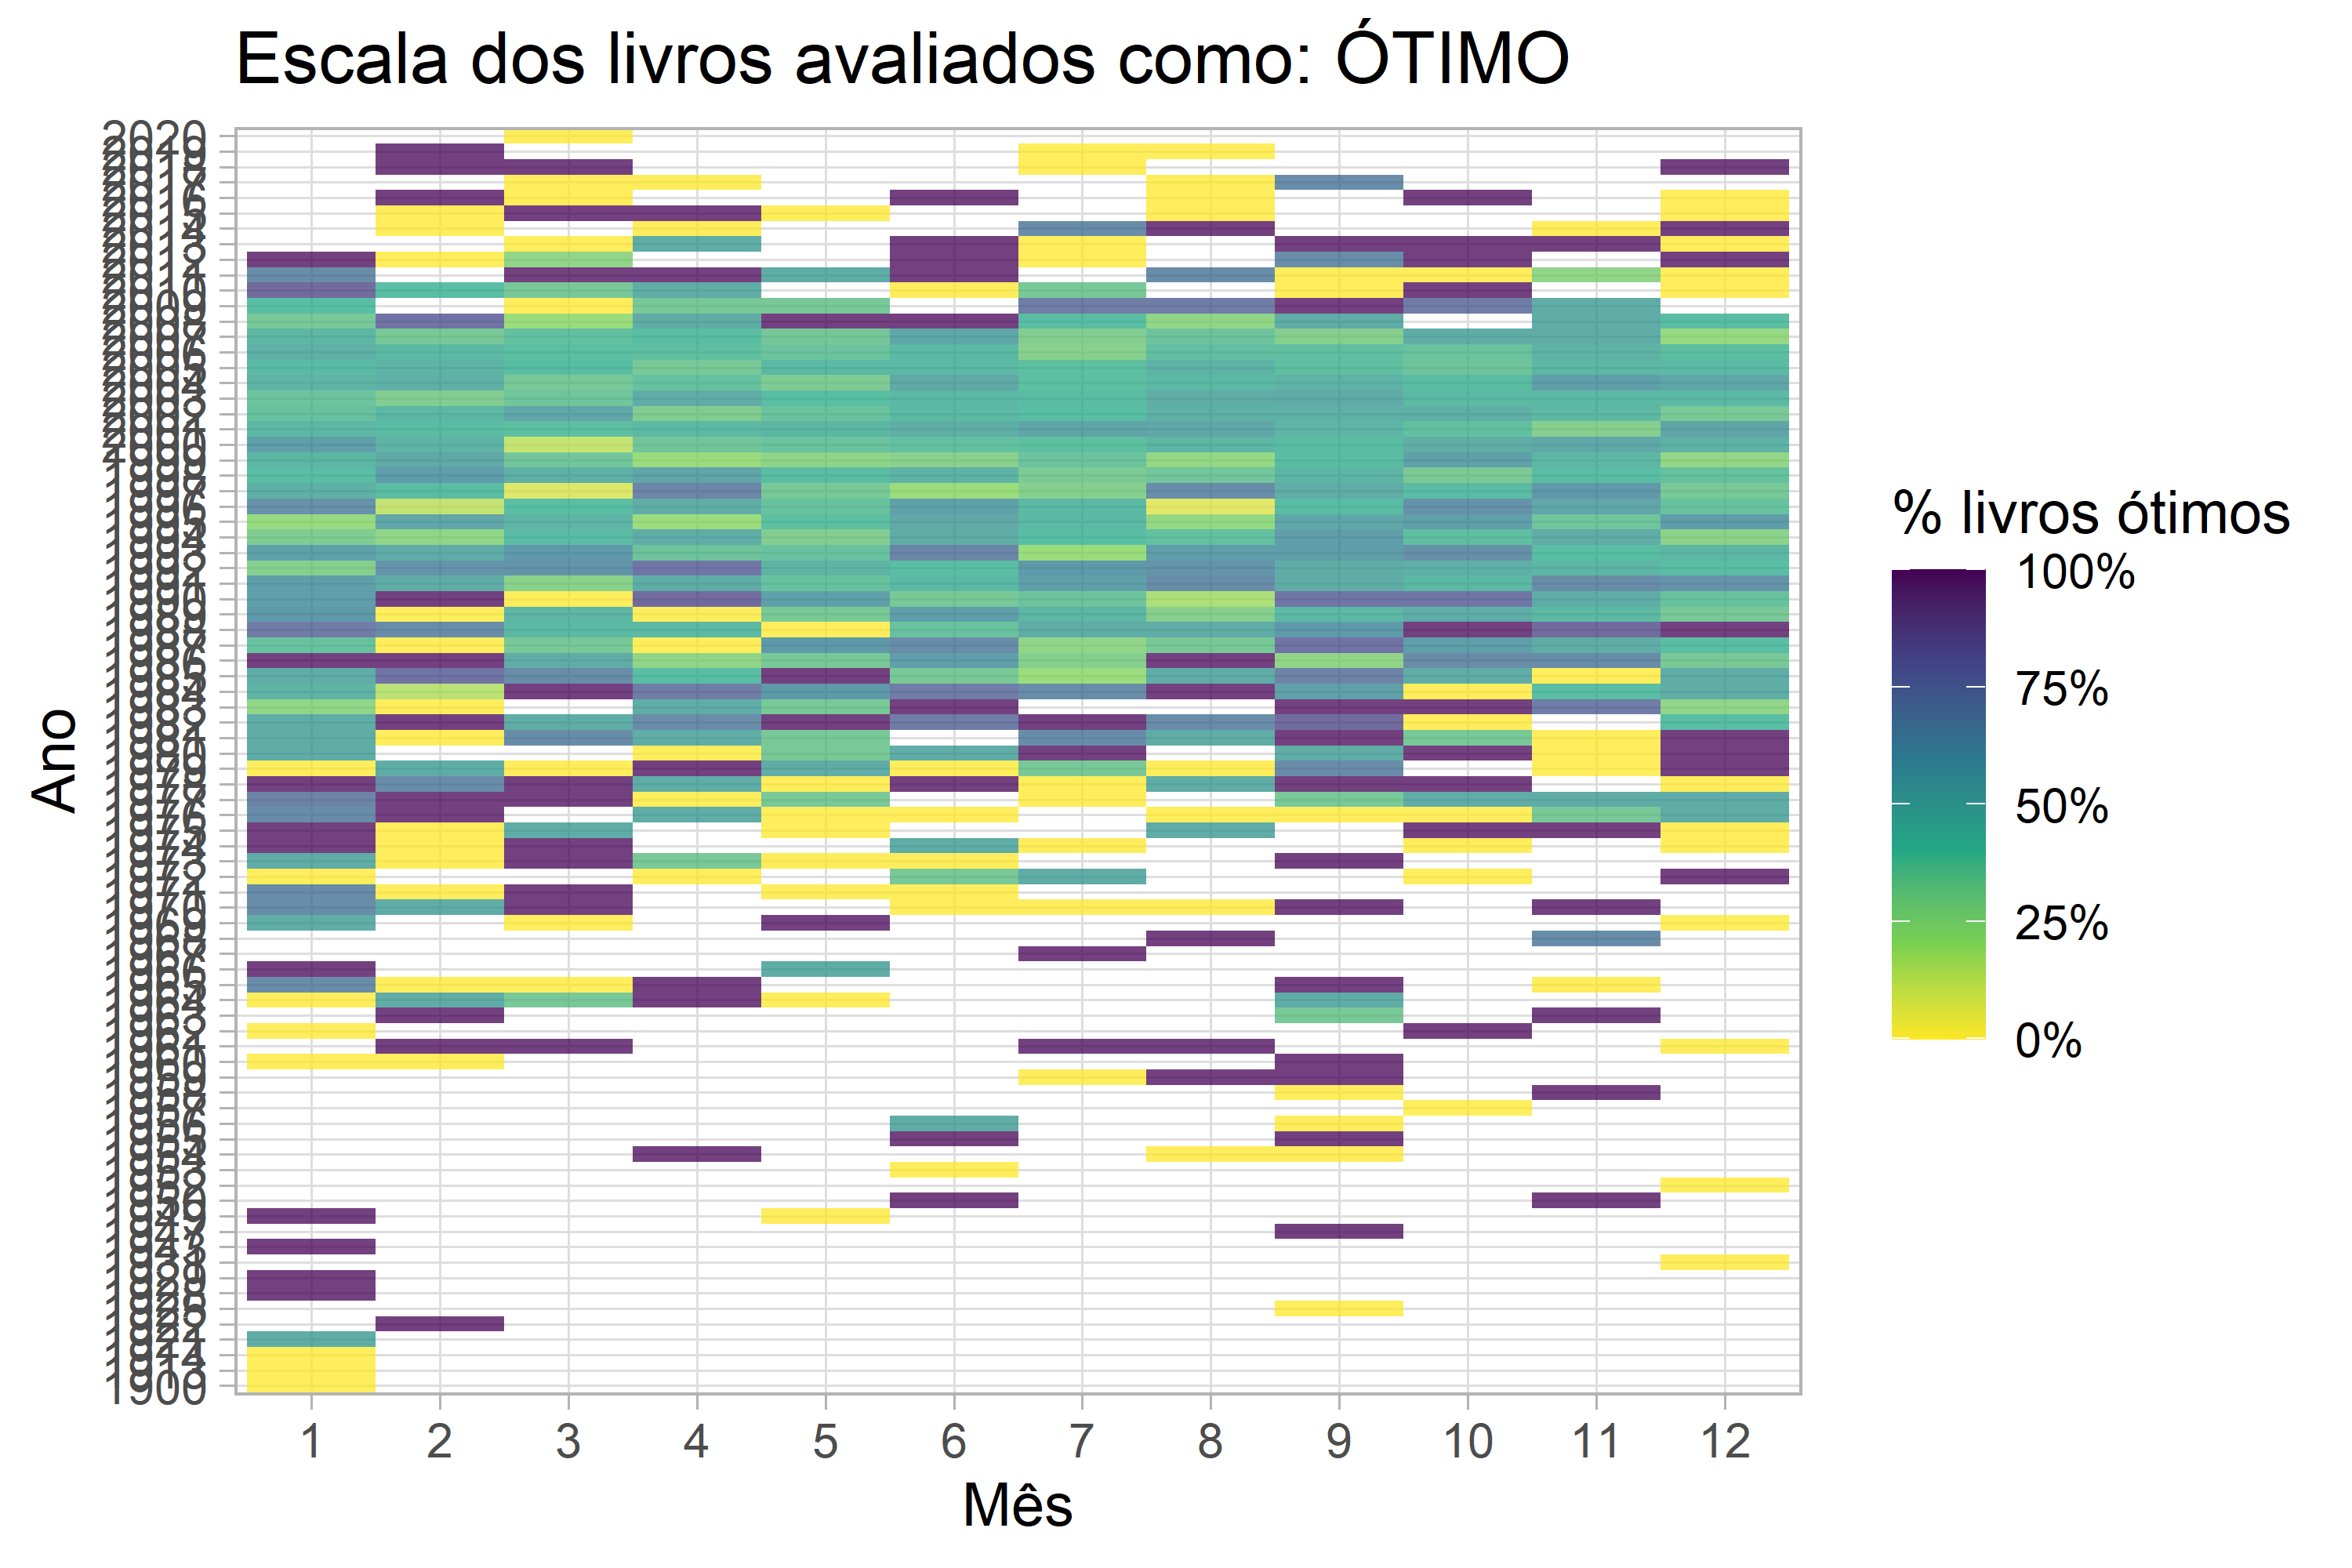
\includegraphics{apresentacao_files/figure-beamer/unnamed-chunk-8-1.png}
\end{frame}

\hypertarget{mais-gruxe1ficos}{%
\subsubsection{Mais gráficos =)}\label{mais-gruxe1ficos}}

\begin{frame}{Mais gráficos =)}
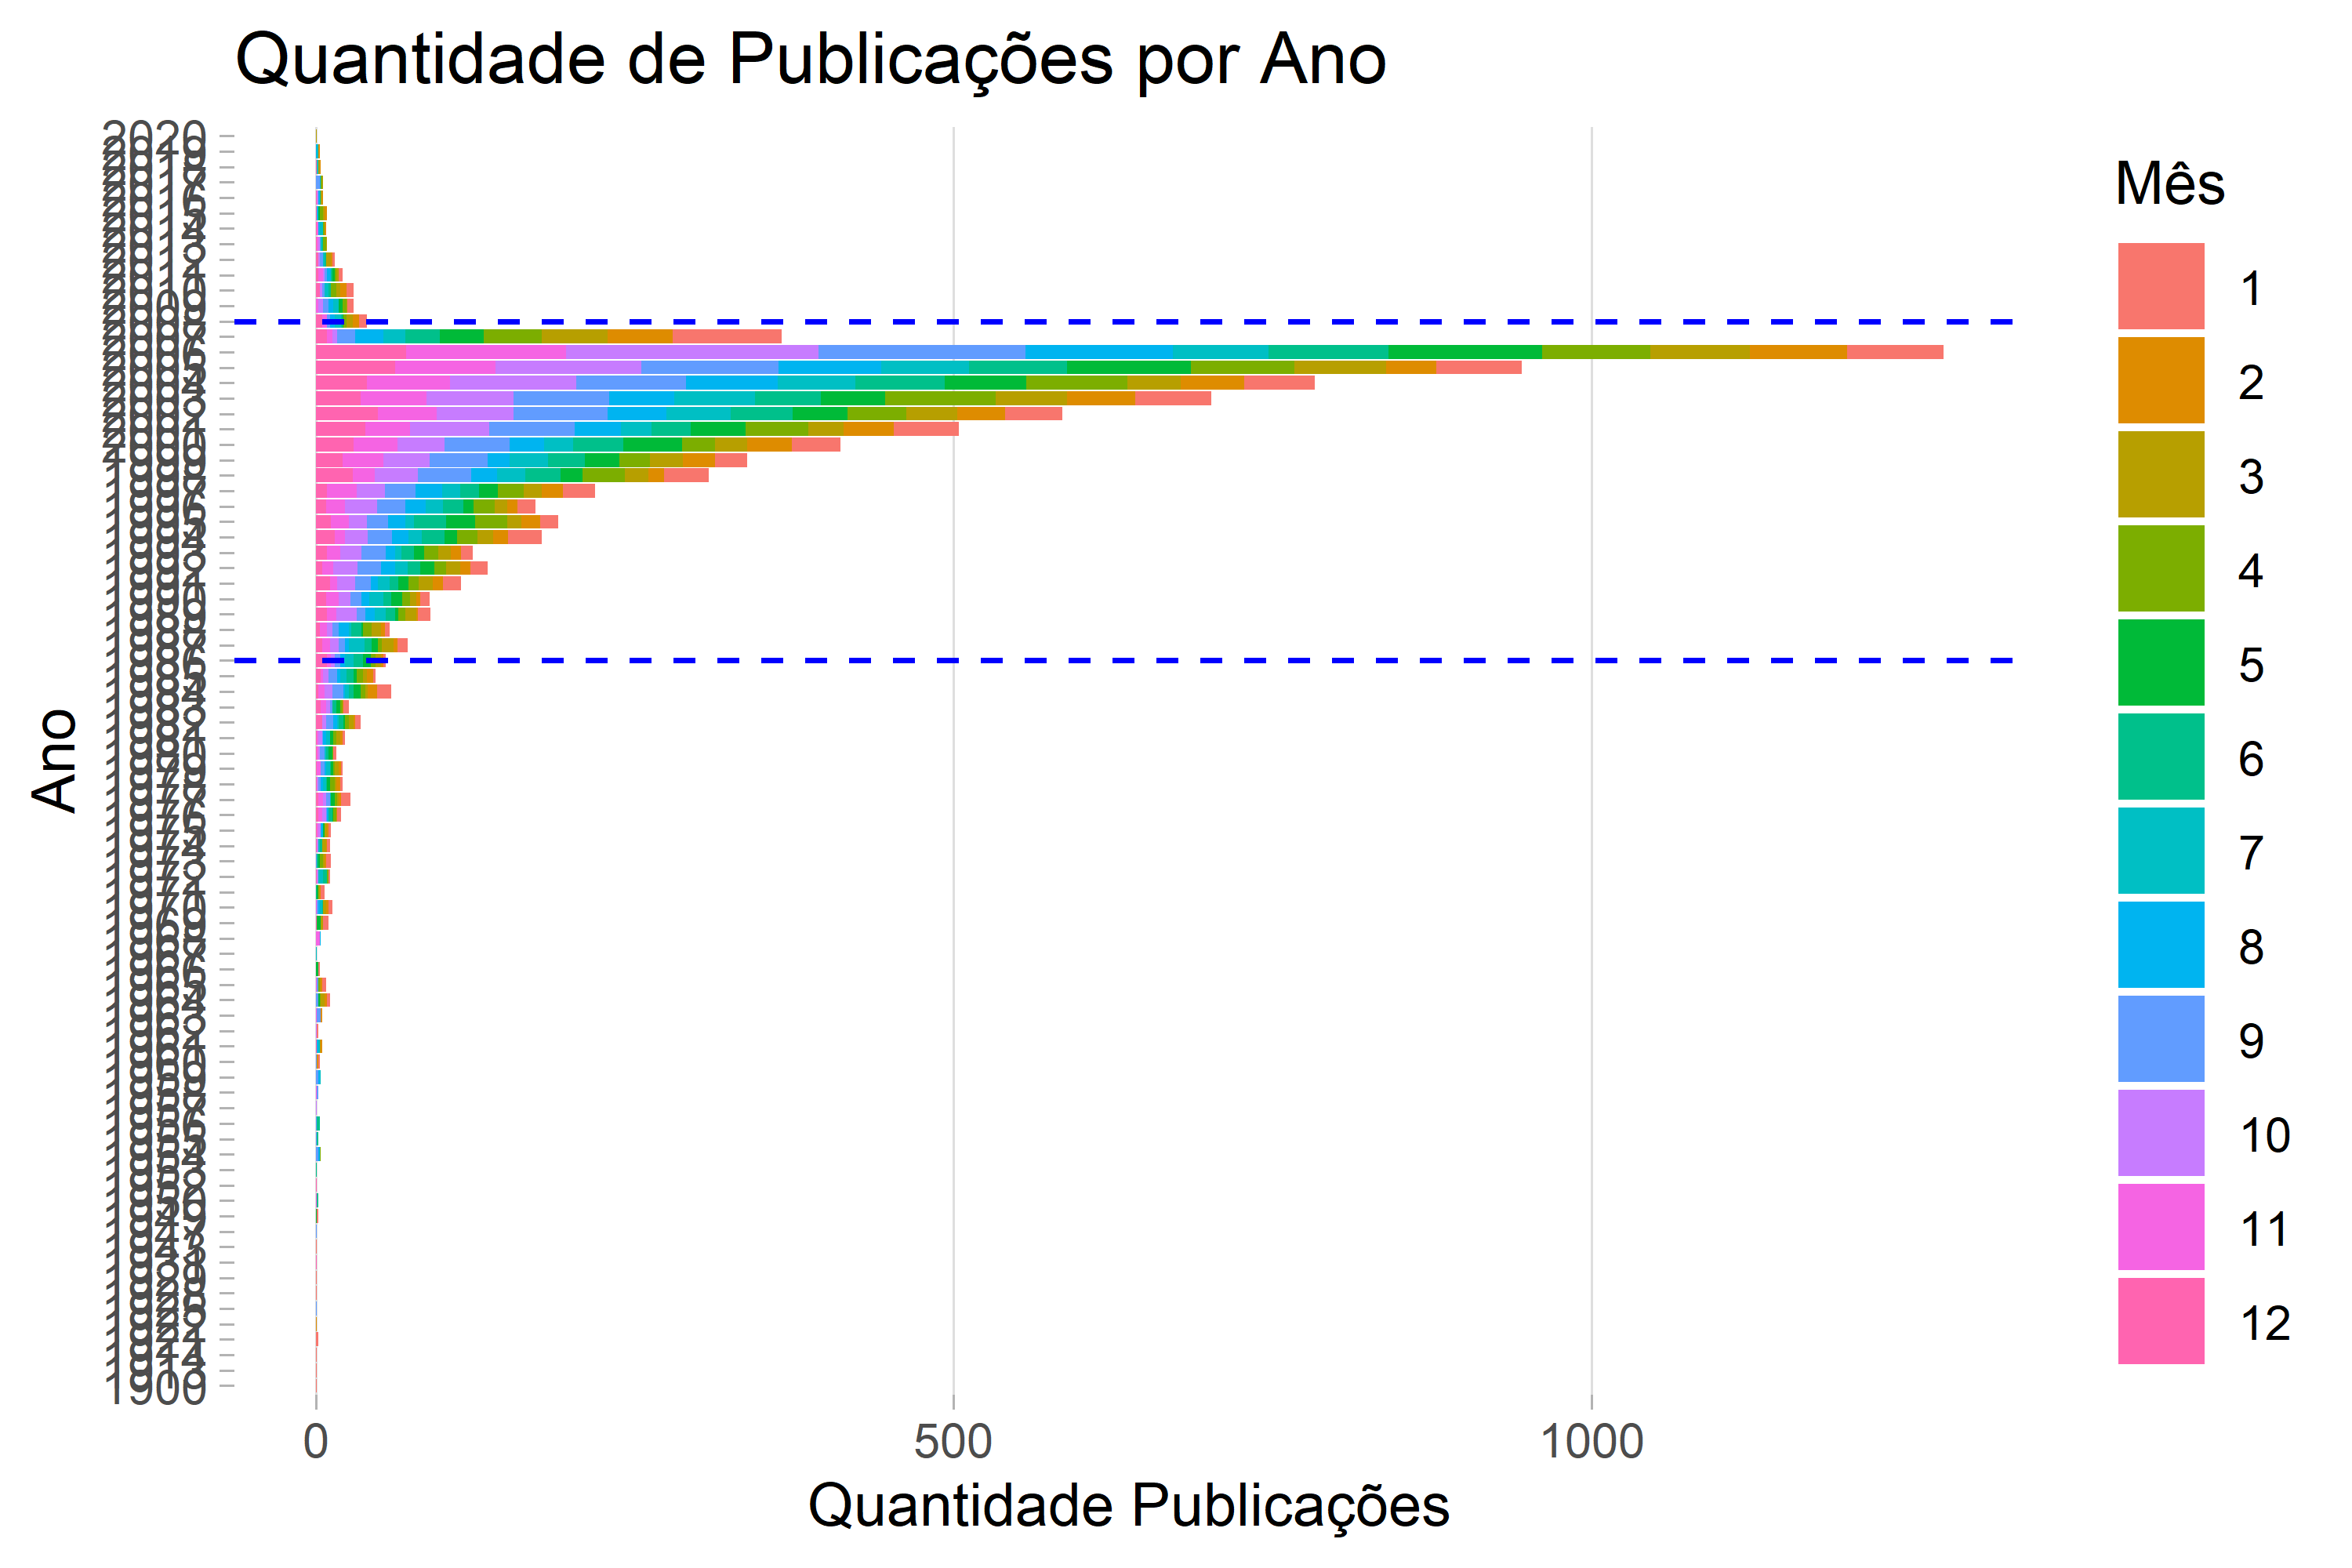
\includegraphics{apresentacao_files/figure-beamer/unnamed-chunk-9-1.png}
\end{frame}

\hypertarget{definindo-filtros}{%
\subsubsection{Definindo Filtros}\label{definindo-filtros}}

\begin{frame}{Definindo Filtros}
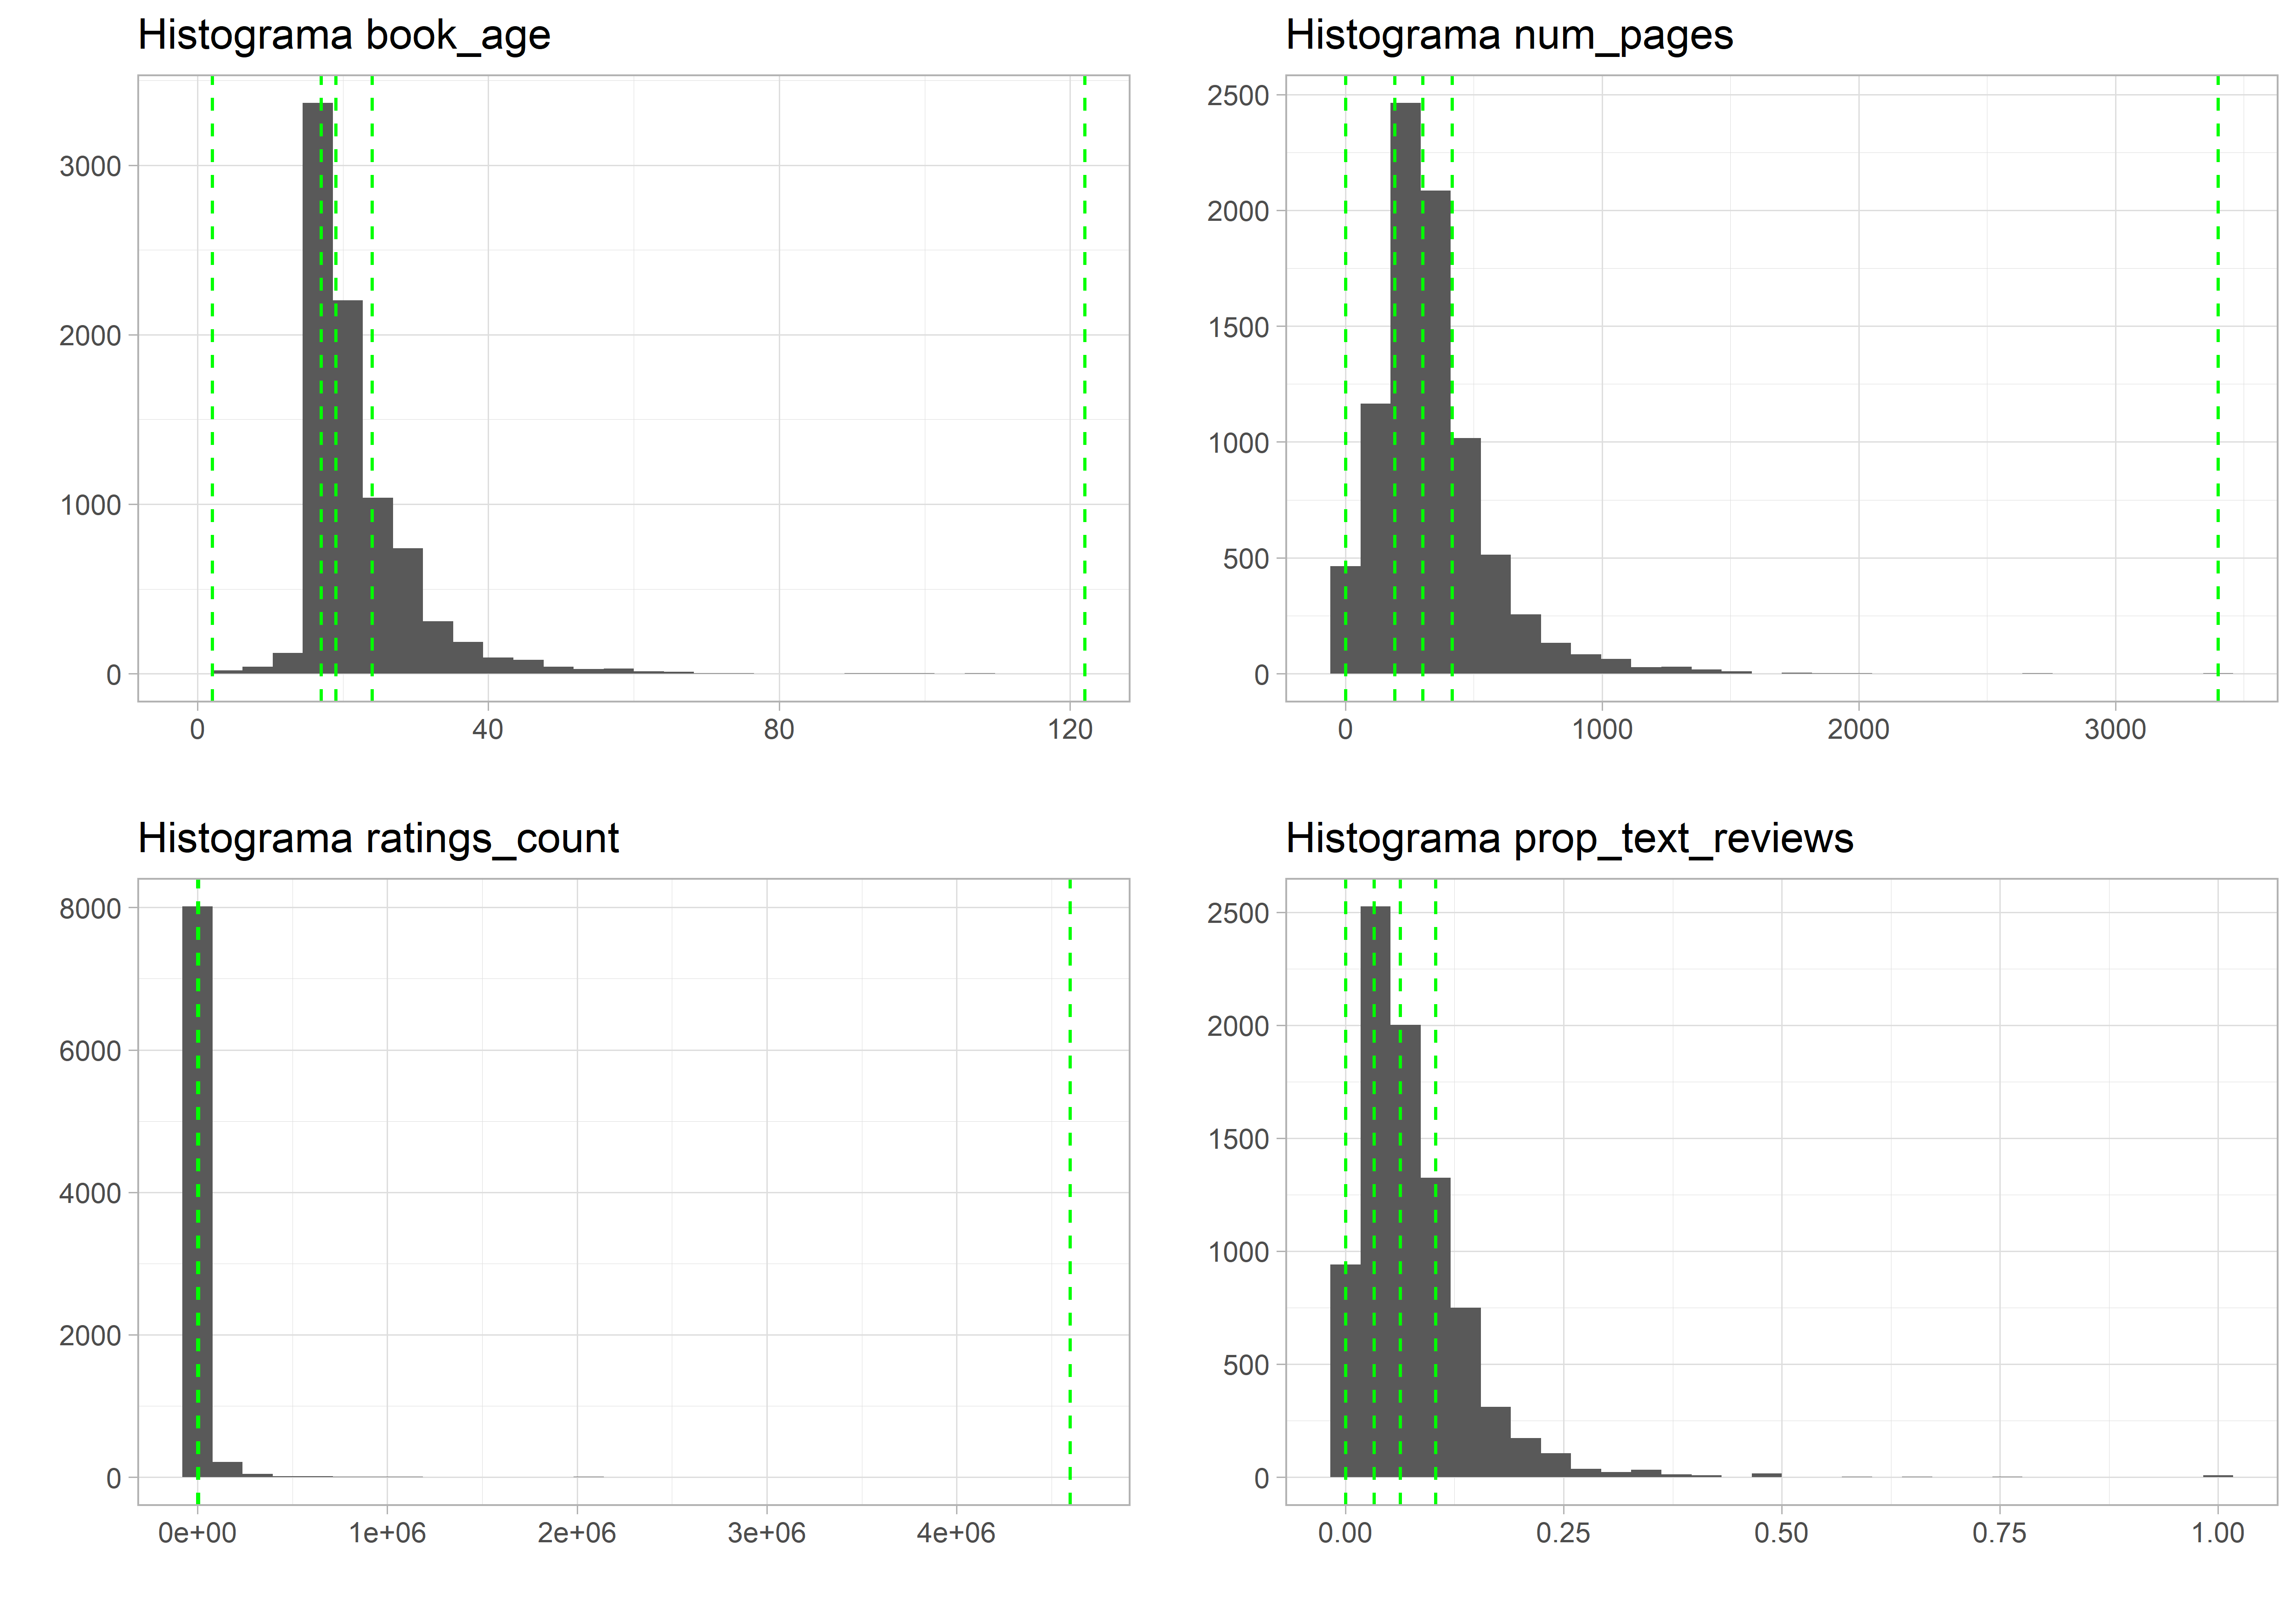
\includegraphics{apresentacao_files/figure-beamer/unnamed-chunk-10-1.png}
\end{frame}

\hypertarget{novo-boxplot-com-filtros-aplicados}{%
\subsubsection{Novo boxplot com filtros
aplicados}\label{novo-boxplot-com-filtros-aplicados}}

\begin{frame}{Novo boxplot com filtros aplicados}
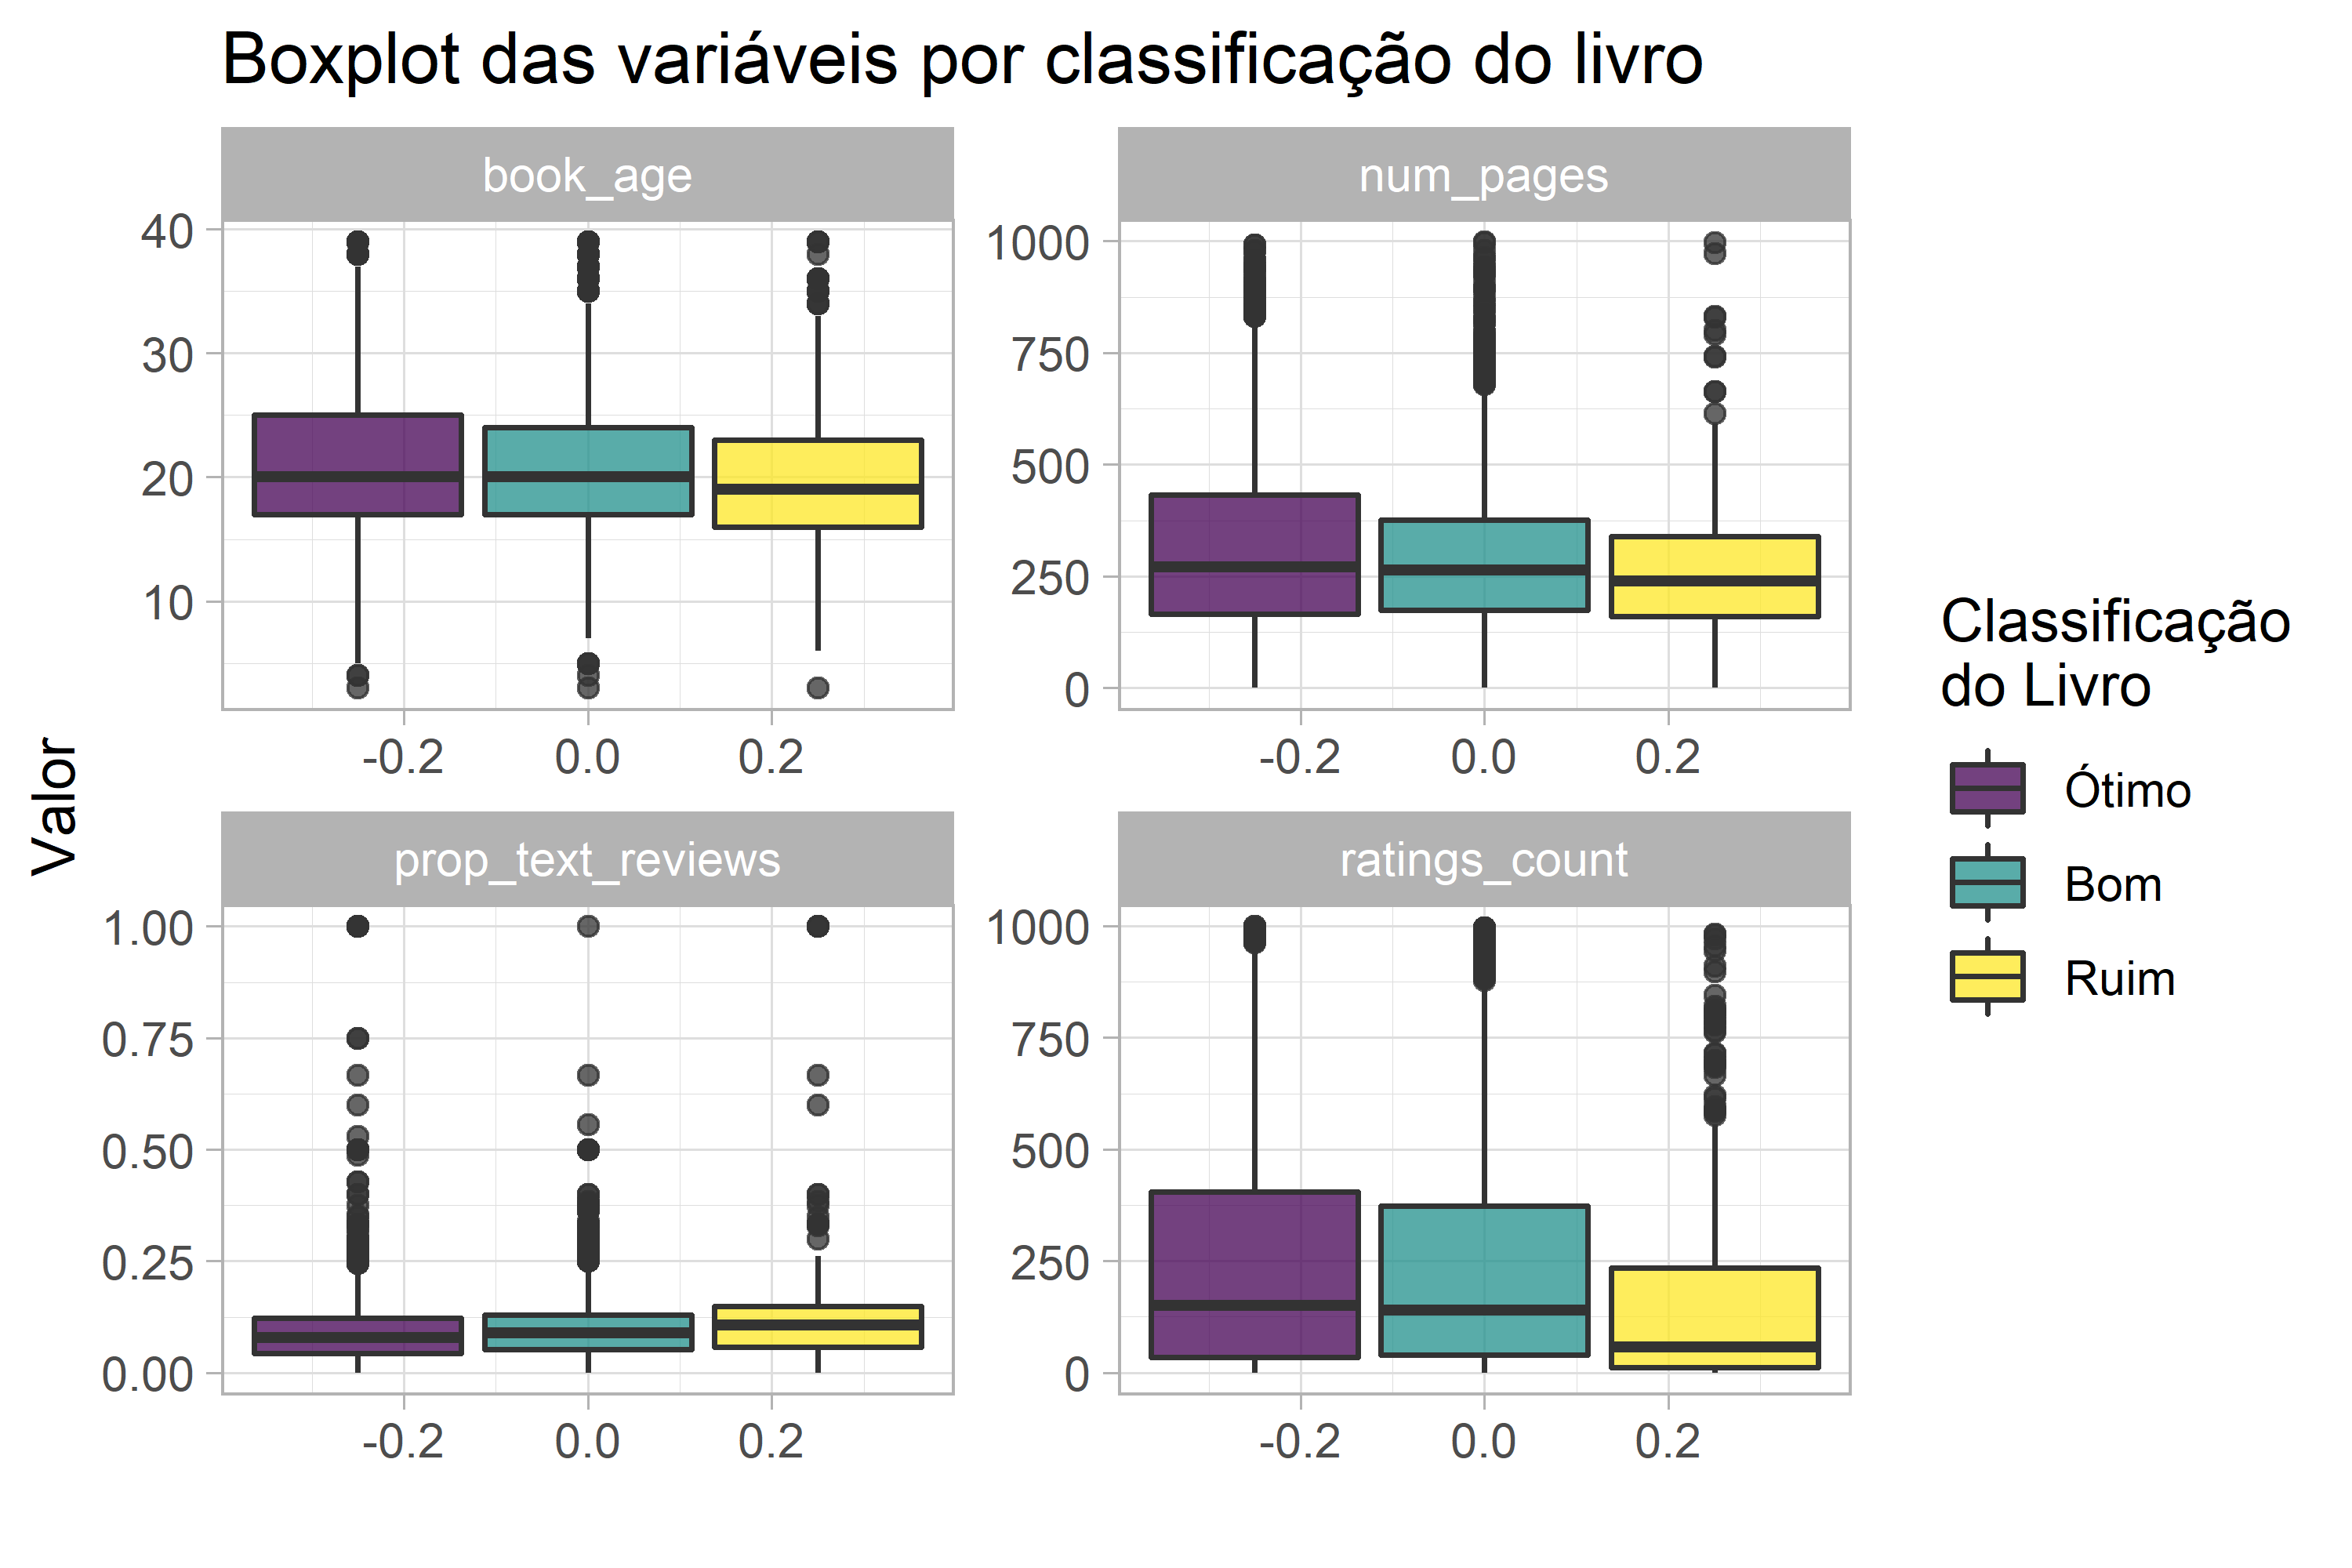
\includegraphics{apresentacao_files/figure-beamer/unnamed-chunk-11-1.png}
\end{frame}

\hypertarget{a-modelagem}{%
\subsection{A modelagem}\label{a-modelagem}}

\begin{frame}[fragile]{A modelagem}
\begin{itemize}
\tightlist
\item
  Com as análises identificamos mudanças necessárias no conjunto de
  dados, demandando nova divisão em \textbf{treino} e \textbf{teste}. Os
  filtros aplicados foram:
\end{itemize}

\begin{table}[H]
\centering
\begin{tabular}{ll}
\toprule
Variável & Filtro\\
\midrule
book\_age & <40\\
num\_pages & <1000\\
rating\_count & <1000\\
prop\_text\_reviews & Nenhum\\
\bottomrule
\end{tabular}
\end{table}

\begin{itemize}
\tightlist
\item
  Posteriormente criamos métricas e \emph{folds} que serão utilizadas
  para \emph{tunar} o módelo:
\end{itemize}

\begin{Shaded}
\begin{Highlighting}[]
\NormalTok{livros\_metricas }\OtherTok{\textless{}{-}} \FunctionTok{metric\_set}\NormalTok{(accuracy, roc\_auc, mn\_log\_loss)}

\FunctionTok{set.seed}\NormalTok{(}\DecValTok{1989}\NormalTok{)}
\NormalTok{livros\_folds }\OtherTok{\textless{}{-}} \FunctionTok{vfold\_cv}\NormalTok{(livros\_treino, }\AttributeTok{strata =}\NormalTok{ book\_rating, }\AttributeTok{v=}\DecValTok{10}\NormalTok{)}
\end{Highlighting}
\end{Shaded}

\begin{itemize}
\tightlist
\item
  E em seguida as demais etapas da modelagem:
\end{itemize}
\end{frame}

\hypertarget{pruxe9-processamento-de-dados}{%
\subsubsection{Pré-Processamento de
Dados}\label{pruxe9-processamento-de-dados}}

\begin{frame}[fragile]{Pré-Processamento de Dados}
\begin{Shaded}
\begin{Highlighting}[]
\NormalTok{livros\_rec }\OtherTok{\textless{}{-}} \FunctionTok{recipe}\NormalTok{(book\_rating }\SpecialCharTok{\textasciitilde{}}\NormalTok{ ., }\AttributeTok{data =}\NormalTok{ livros\_treino) }\SpecialCharTok{\%\textgreater{}\%}
\NormalTok{  themis}\SpecialCharTok{::}\FunctionTok{step\_downsample}\NormalTok{(book\_rating) }\SpecialCharTok{\%\textgreater{}\%} 
  \FunctionTok{step\_date}\NormalTok{(publication\_date, }\AttributeTok{features =} \FunctionTok{c}\NormalTok{(}\StringTok{"month"}\NormalTok{), }
            \AttributeTok{keep\_original\_cols =} \ConstantTok{FALSE}\NormalTok{) }\SpecialCharTok{\%\textgreater{}\%}
  \FunctionTok{step\_dummy}\NormalTok{(}\FunctionTok{all\_nominal\_predictors}\NormalTok{(), }\AttributeTok{one\_hot =} \ConstantTok{TRUE}\NormalTok{) }\SpecialCharTok{\%\textgreater{}\%}
  \FunctionTok{step\_zv}\NormalTok{(}\FunctionTok{all\_predictors}\NormalTok{()) }\SpecialCharTok{\%\textgreater{}\%} 
  \FunctionTok{prep}\NormalTok{()}
\end{Highlighting}
\end{Shaded}
\end{frame}

\hypertarget{grid-de-procura-e-de-parada-antecipada}{%
\subsubsection{Grid de Procura e de Parada
antecipada}\label{grid-de-procura-e-de-parada-antecipada}}

\begin{frame}[fragile]{Grid de Procura e de Parada antecipada}
\begin{Shaded}
\begin{Highlighting}[]
\NormalTok{stopping\_spec }\OtherTok{\textless{}{-}}
  \FunctionTok{boost\_tree}\NormalTok{(}
    \AttributeTok{trees =} \DecValTok{500}\NormalTok{,}
    \AttributeTok{mtry =} \FunctionTok{tune}\NormalTok{(),}
    \AttributeTok{learn\_rate =} \FunctionTok{tune}\NormalTok{(),}
    \AttributeTok{stop\_iter =} \FunctionTok{tune}\NormalTok{()}
\NormalTok{  ) }\SpecialCharTok{\%\textgreater{}\%}
  \FunctionTok{set\_engine}\NormalTok{(}\StringTok{"xgboost"}\NormalTok{, }\AttributeTok{validation =} \FloatTok{0.2}\NormalTok{) }\SpecialCharTok{\%\textgreater{}\%}
  \FunctionTok{set\_mode}\NormalTok{(}\StringTok{"classification"}\NormalTok{)}
\NormalTok{stopping\_grid }\OtherTok{\textless{}{-}}
  \FunctionTok{grid\_latin\_hypercube}\NormalTok{(}
    \FunctionTok{mtry}\NormalTok{(}\AttributeTok{range =} \FunctionTok{c}\NormalTok{(}\DecValTok{5}\NormalTok{, }\DecValTok{18}\NormalTok{)),}
    \FunctionTok{learn\_rate}\NormalTok{(}\AttributeTok{range =} \FunctionTok{c}\NormalTok{(}\SpecialCharTok{{-}}\DecValTok{5}\NormalTok{, }\SpecialCharTok{{-}}\DecValTok{1}\NormalTok{)), }
    \FunctionTok{stop\_iter}\NormalTok{(}\AttributeTok{range =} \FunctionTok{c}\NormalTok{(}\DecValTok{10}\NormalTok{, }\DecValTok{50}\NormalTok{)), }
    \AttributeTok{size =} \DecValTok{10}
\NormalTok{  )}
\NormalTok{early\_stop\_wf }\OtherTok{\textless{}{-}} \FunctionTok{workflow}\NormalTok{(livros\_rec, stopping\_spec)}
\end{Highlighting}
\end{Shaded}
\end{frame}

\begin{frame}[fragile]{Definido os grids de procura e parada, é hora de
\textbf{TUNAR} o modelo!}
\protect\hypertarget{definido-os-grids-de-procura-e-parada-uxe9-hora-de-tunar-o-modelo}{}
\begin{Shaded}
\begin{Highlighting}[]
\NormalTok{doParallel}\SpecialCharTok{::}\FunctionTok{registerDoParallel}\NormalTok{()}
\FunctionTok{set.seed}\NormalTok{(}\DecValTok{2022}\NormalTok{)}
\NormalTok{stopping\_rs }\OtherTok{\textless{}{-}} \FunctionTok{tune\_grid}\NormalTok{(}
\NormalTok{  early\_stop\_wf,}
\NormalTok{  livros\_folds,}
  \AttributeTok{grid =}\NormalTok{ stopping\_grid,}
  \AttributeTok{metrics =}\NormalTok{ livros\_metricas}
\NormalTok{)}
\end{Highlighting}
\end{Shaded}
\end{frame}

\hypertarget{resultados}{%
\subsection{Resultados}\label{resultados}}

\hypertarget{interauxe7uxf5es-e-taxa-de-aprendizagem}{%
\subsubsection{Interações e Taxa de
Aprendizagem}\label{interauxe7uxf5es-e-taxa-de-aprendizagem}}

\begin{frame}{Interações e Taxa de Aprendizagem}
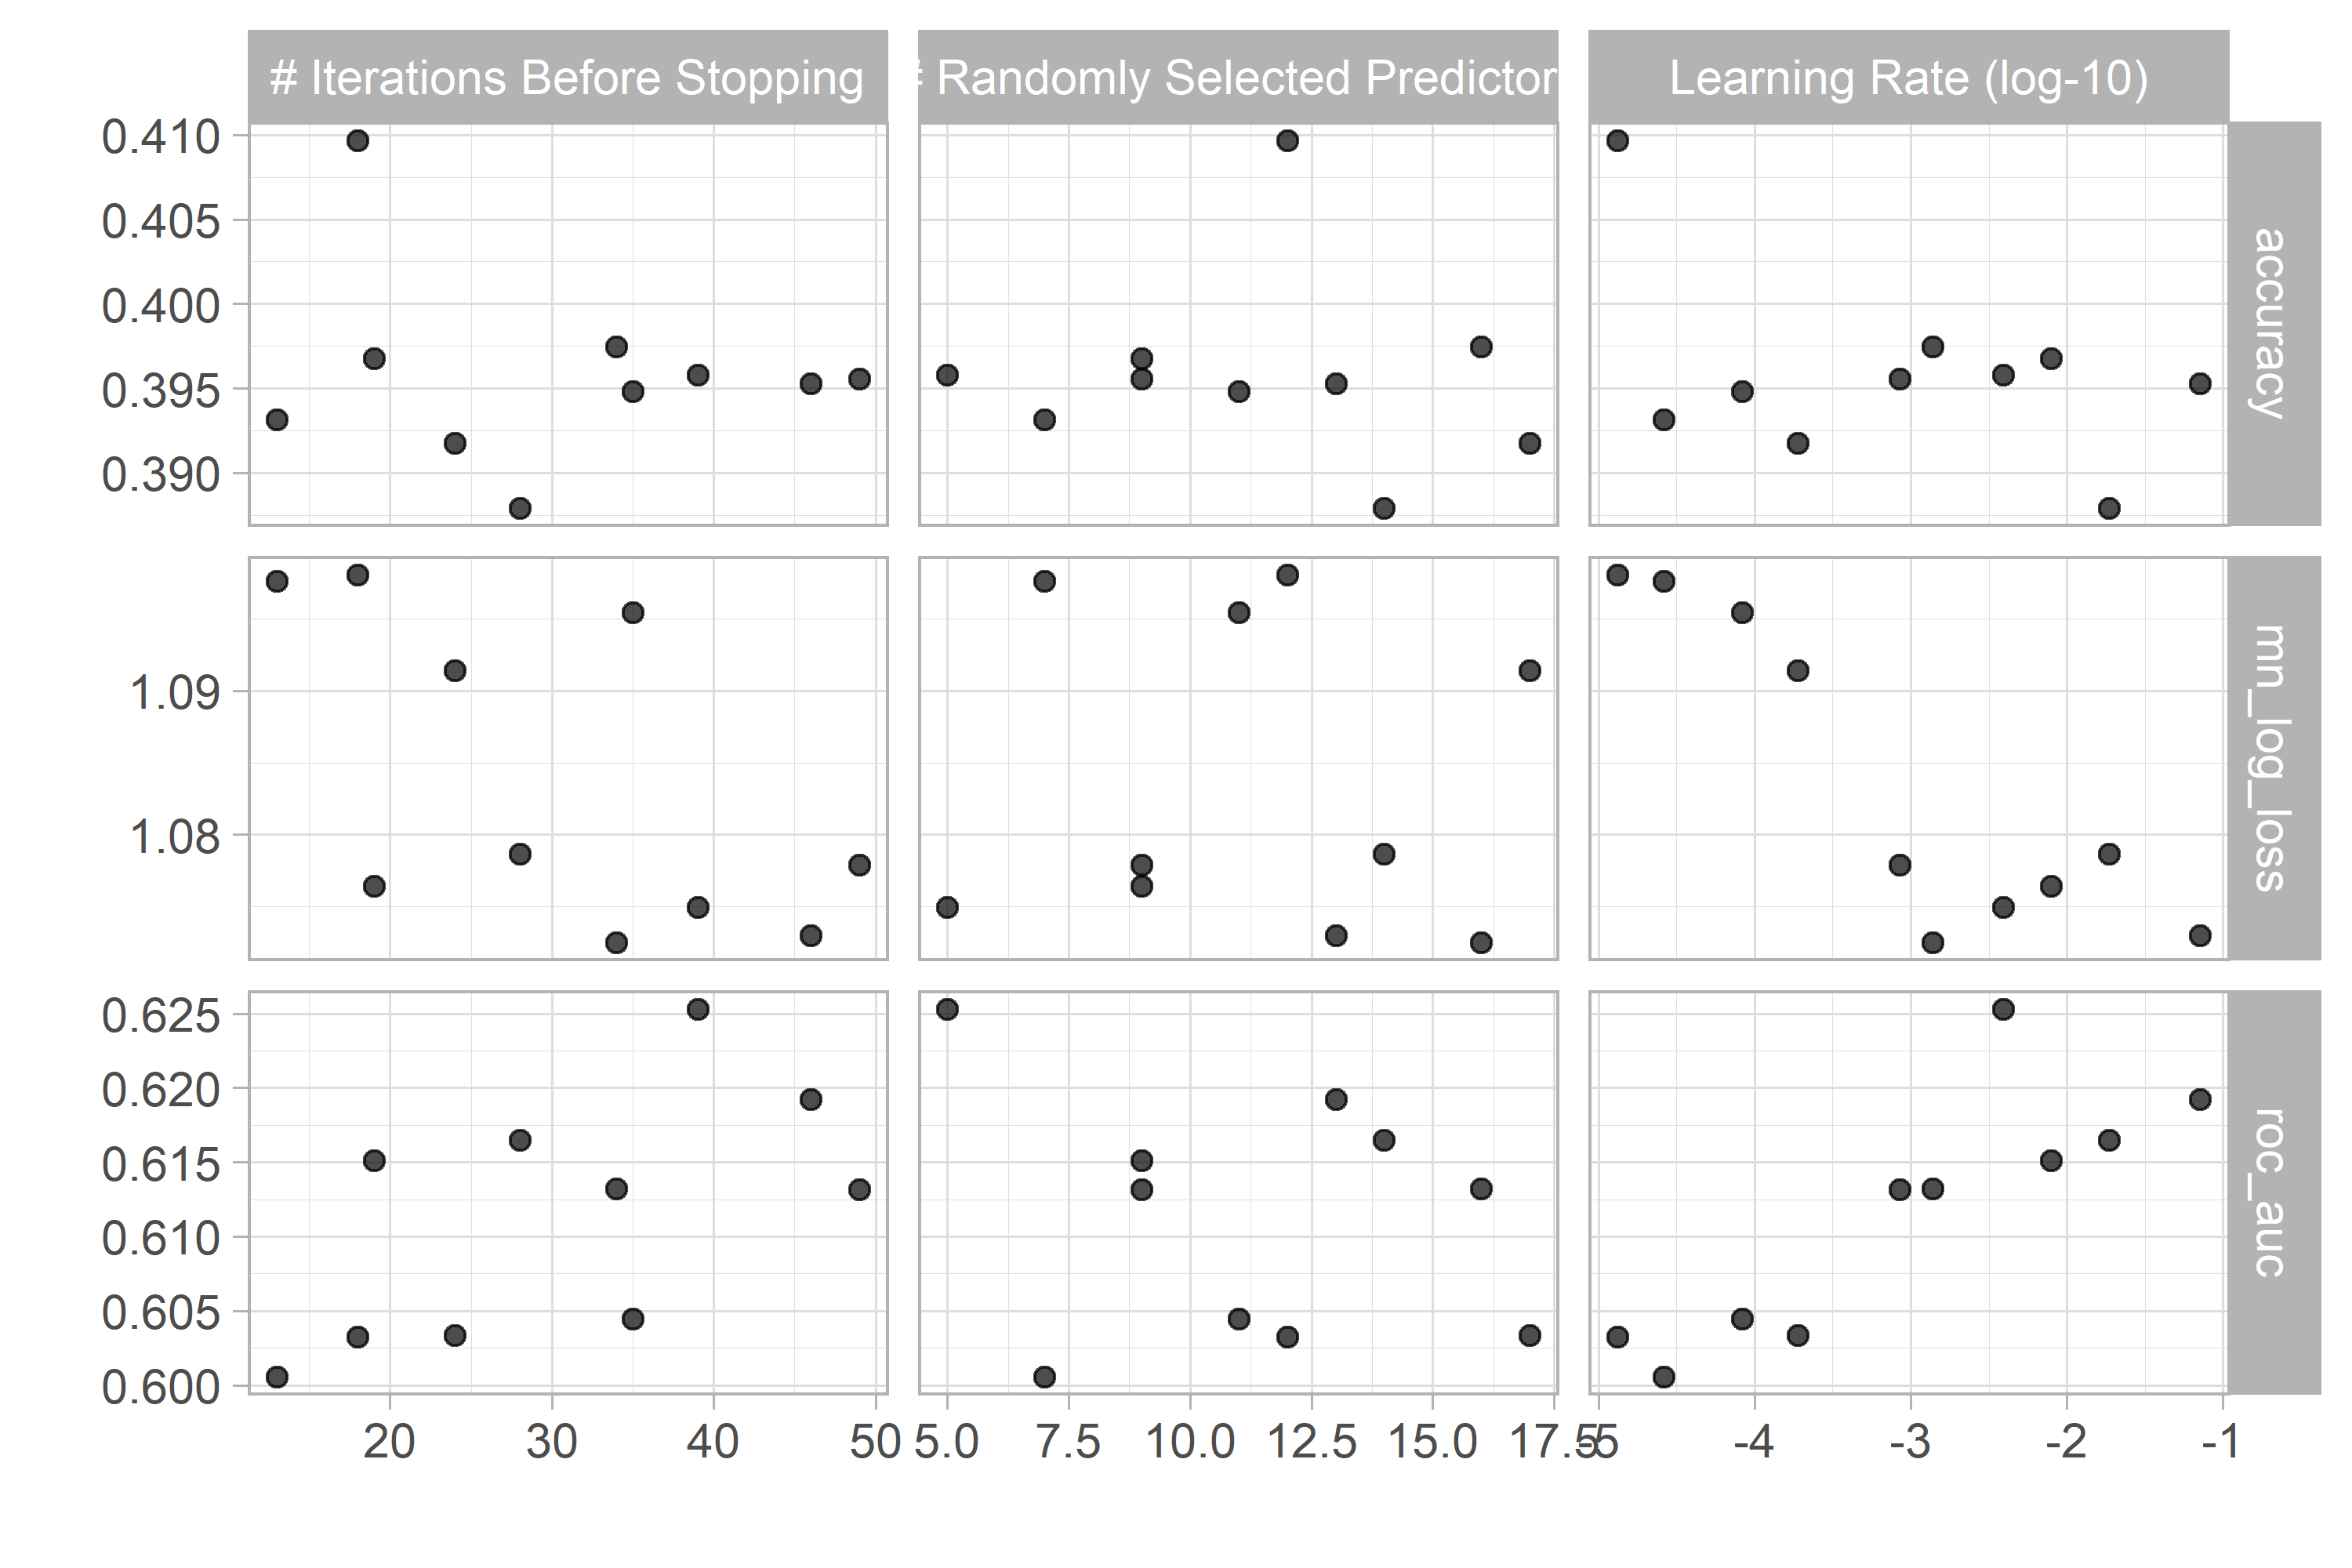
\includegraphics{apresentacao_files/figure-beamer/unnamed-chunk-17-1.png}
\end{frame}

\hypertarget{avaliauxe7uxe3o-do-modelo}{%
\subsubsection{Avaliação do modelo}\label{avaliauxe7uxe3o-do-modelo}}

\begin{frame}[fragile]{Avaliação do modelo}
\begin{itemize}
\tightlist
\item
  Avaliando o melhor resultado de acordo com \textbf{mn\_log\_loss},
  pois é com ele que acompanhamos a capacidade de aprendizagem do
  modelo:
\end{itemize}

\begin{Shaded}
\begin{Highlighting}[]
\FunctionTok{show\_best}\NormalTok{(stopping\_rs, }\AttributeTok{metric =} \StringTok{"mn\_log\_loss"}\NormalTok{)}
\end{Highlighting}
\end{Shaded}

\begin{table}[H]
\centering
\begin{tabular}{rrrrrrl}
\toprule
mtry & learn\_rate & stop\_iter & mean & n & std\_err & .config\\
\midrule
17 & 0.0286 & 17 & 1.069 & 10 & 0.0059 & Preprocessor1\_Model10\\
14 & 0.0910 & 23 & 1.072 & 10 & 0.0043 & Preprocessor1\_Model09\\
16 & 0.0046 & 21 & 1.073 & 10 & 0.0050 & Preprocessor1\_Model01\\
8 & 0.0108 & 40 & 1.073 & 10 & 0.0028 & Preprocessor1\_Model05\\
12 & 0.0019 & 11 & 1.073 & 10 & 0.0039 & Preprocessor1\_Model04\\
\bottomrule
\end{tabular}
\end{table}

\begin{itemize}
\tightlist
\item
  Em seguida realizamos o modelo final e avaliamos as demais métricas:
\end{itemize}

\begin{Shaded}
\begin{Highlighting}[]
\NormalTok{stopping\_fit }\OtherTok{\textless{}{-}}\NormalTok{ early\_stop\_wf }\SpecialCharTok{\%\textgreater{}\%}
  \FunctionTok{finalize\_workflow}\NormalTok{(}\FunctionTok{select\_best}\NormalTok{(stopping\_rs, }\StringTok{"mn\_log\_loss"}\NormalTok{)) }\SpecialCharTok{\%\textgreater{}\%}
  \FunctionTok{last\_fit}\NormalTok{(livros\_split)}

\FunctionTok{collect\_metrics}\NormalTok{(stopping\_fit)}
\end{Highlighting}
\end{Shaded}

\begin{table}[H]
\centering
\begin{tabular}{llrl}
\toprule
.metric & .estimator & .estimate & .config\\
\midrule
accuracy & multiclass & 0.4011 & Preprocessor1\_Model1\\
roc\_auc & hand\_till & 0.6091 & Preprocessor1\_Model1\\
\bottomrule
\end{tabular}
\end{table}
\end{frame}

\hypertarget{variuxe1veis-vip}{%
\subsubsection{Variáveis VIP}\label{variuxe1veis-vip}}

\begin{frame}{Variáveis VIP}
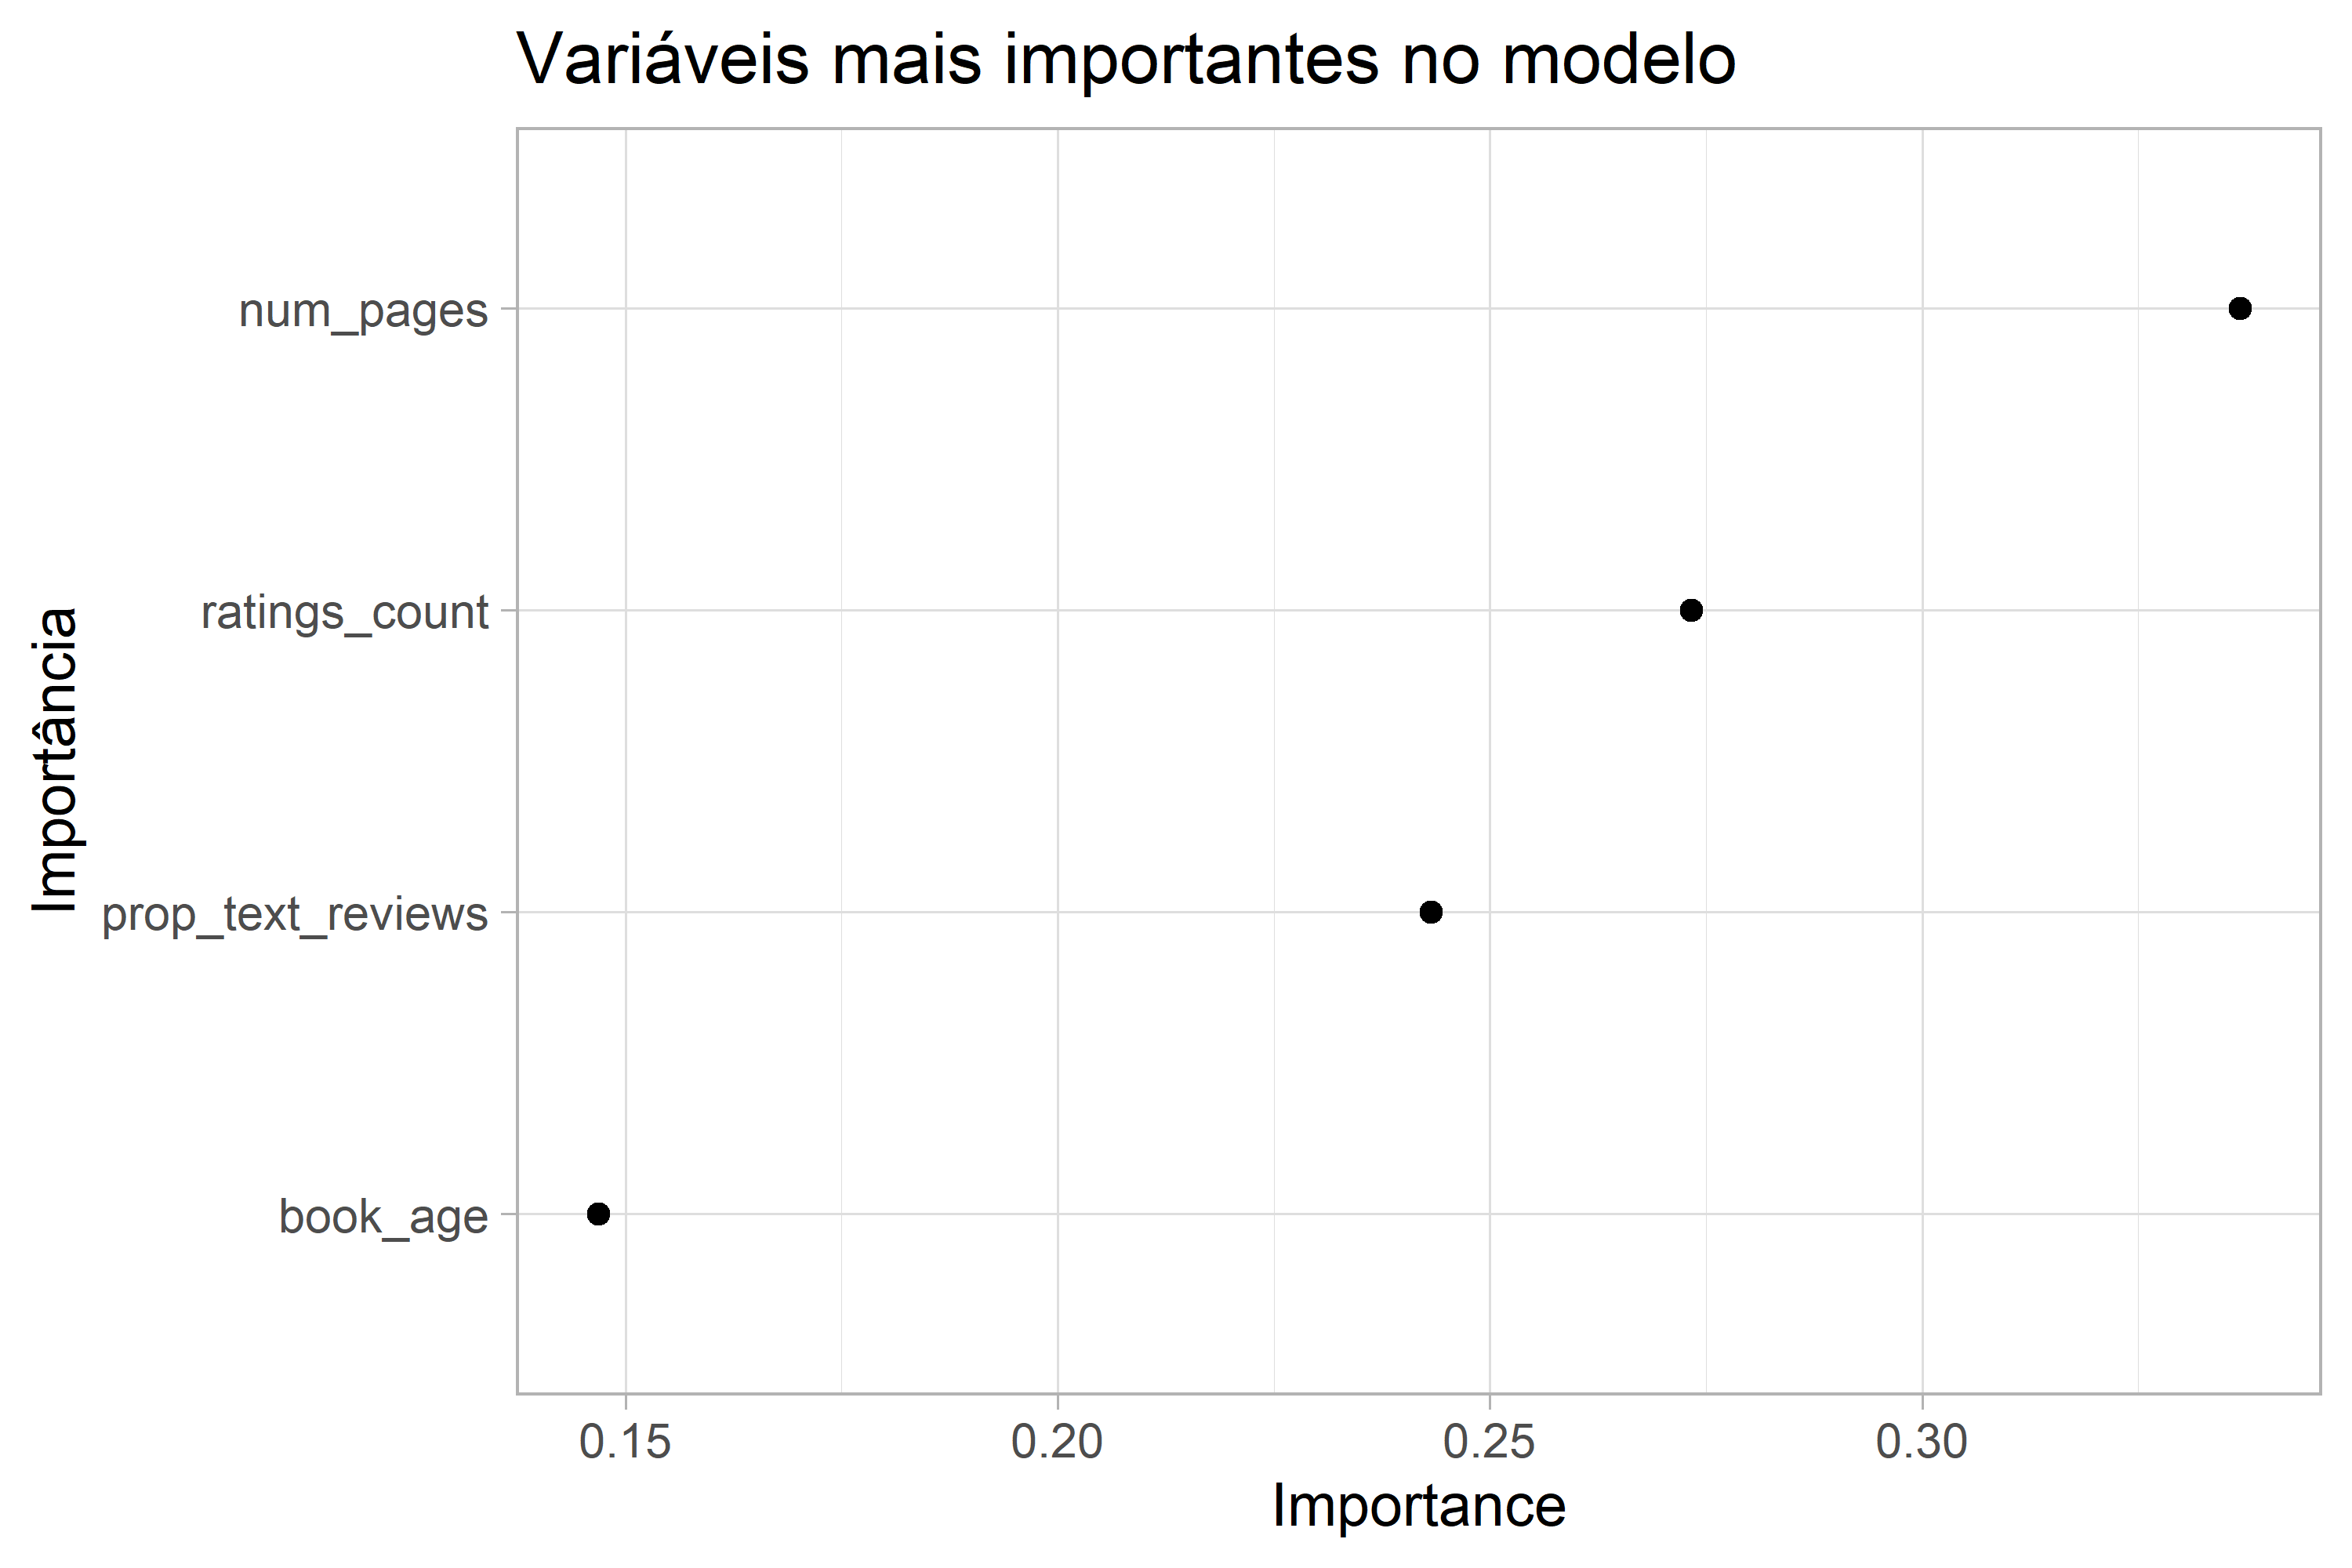
\includegraphics{apresentacao_files/figure-beamer/unnamed-chunk-22-1.png}
\end{frame}

\hypertarget{heatmap}{%
\subsubsection{\texorpdfstring{\emph{Heatmap}}{Heatmap}}\label{heatmap}}

\begin{frame}{\emph{Heatmap}}
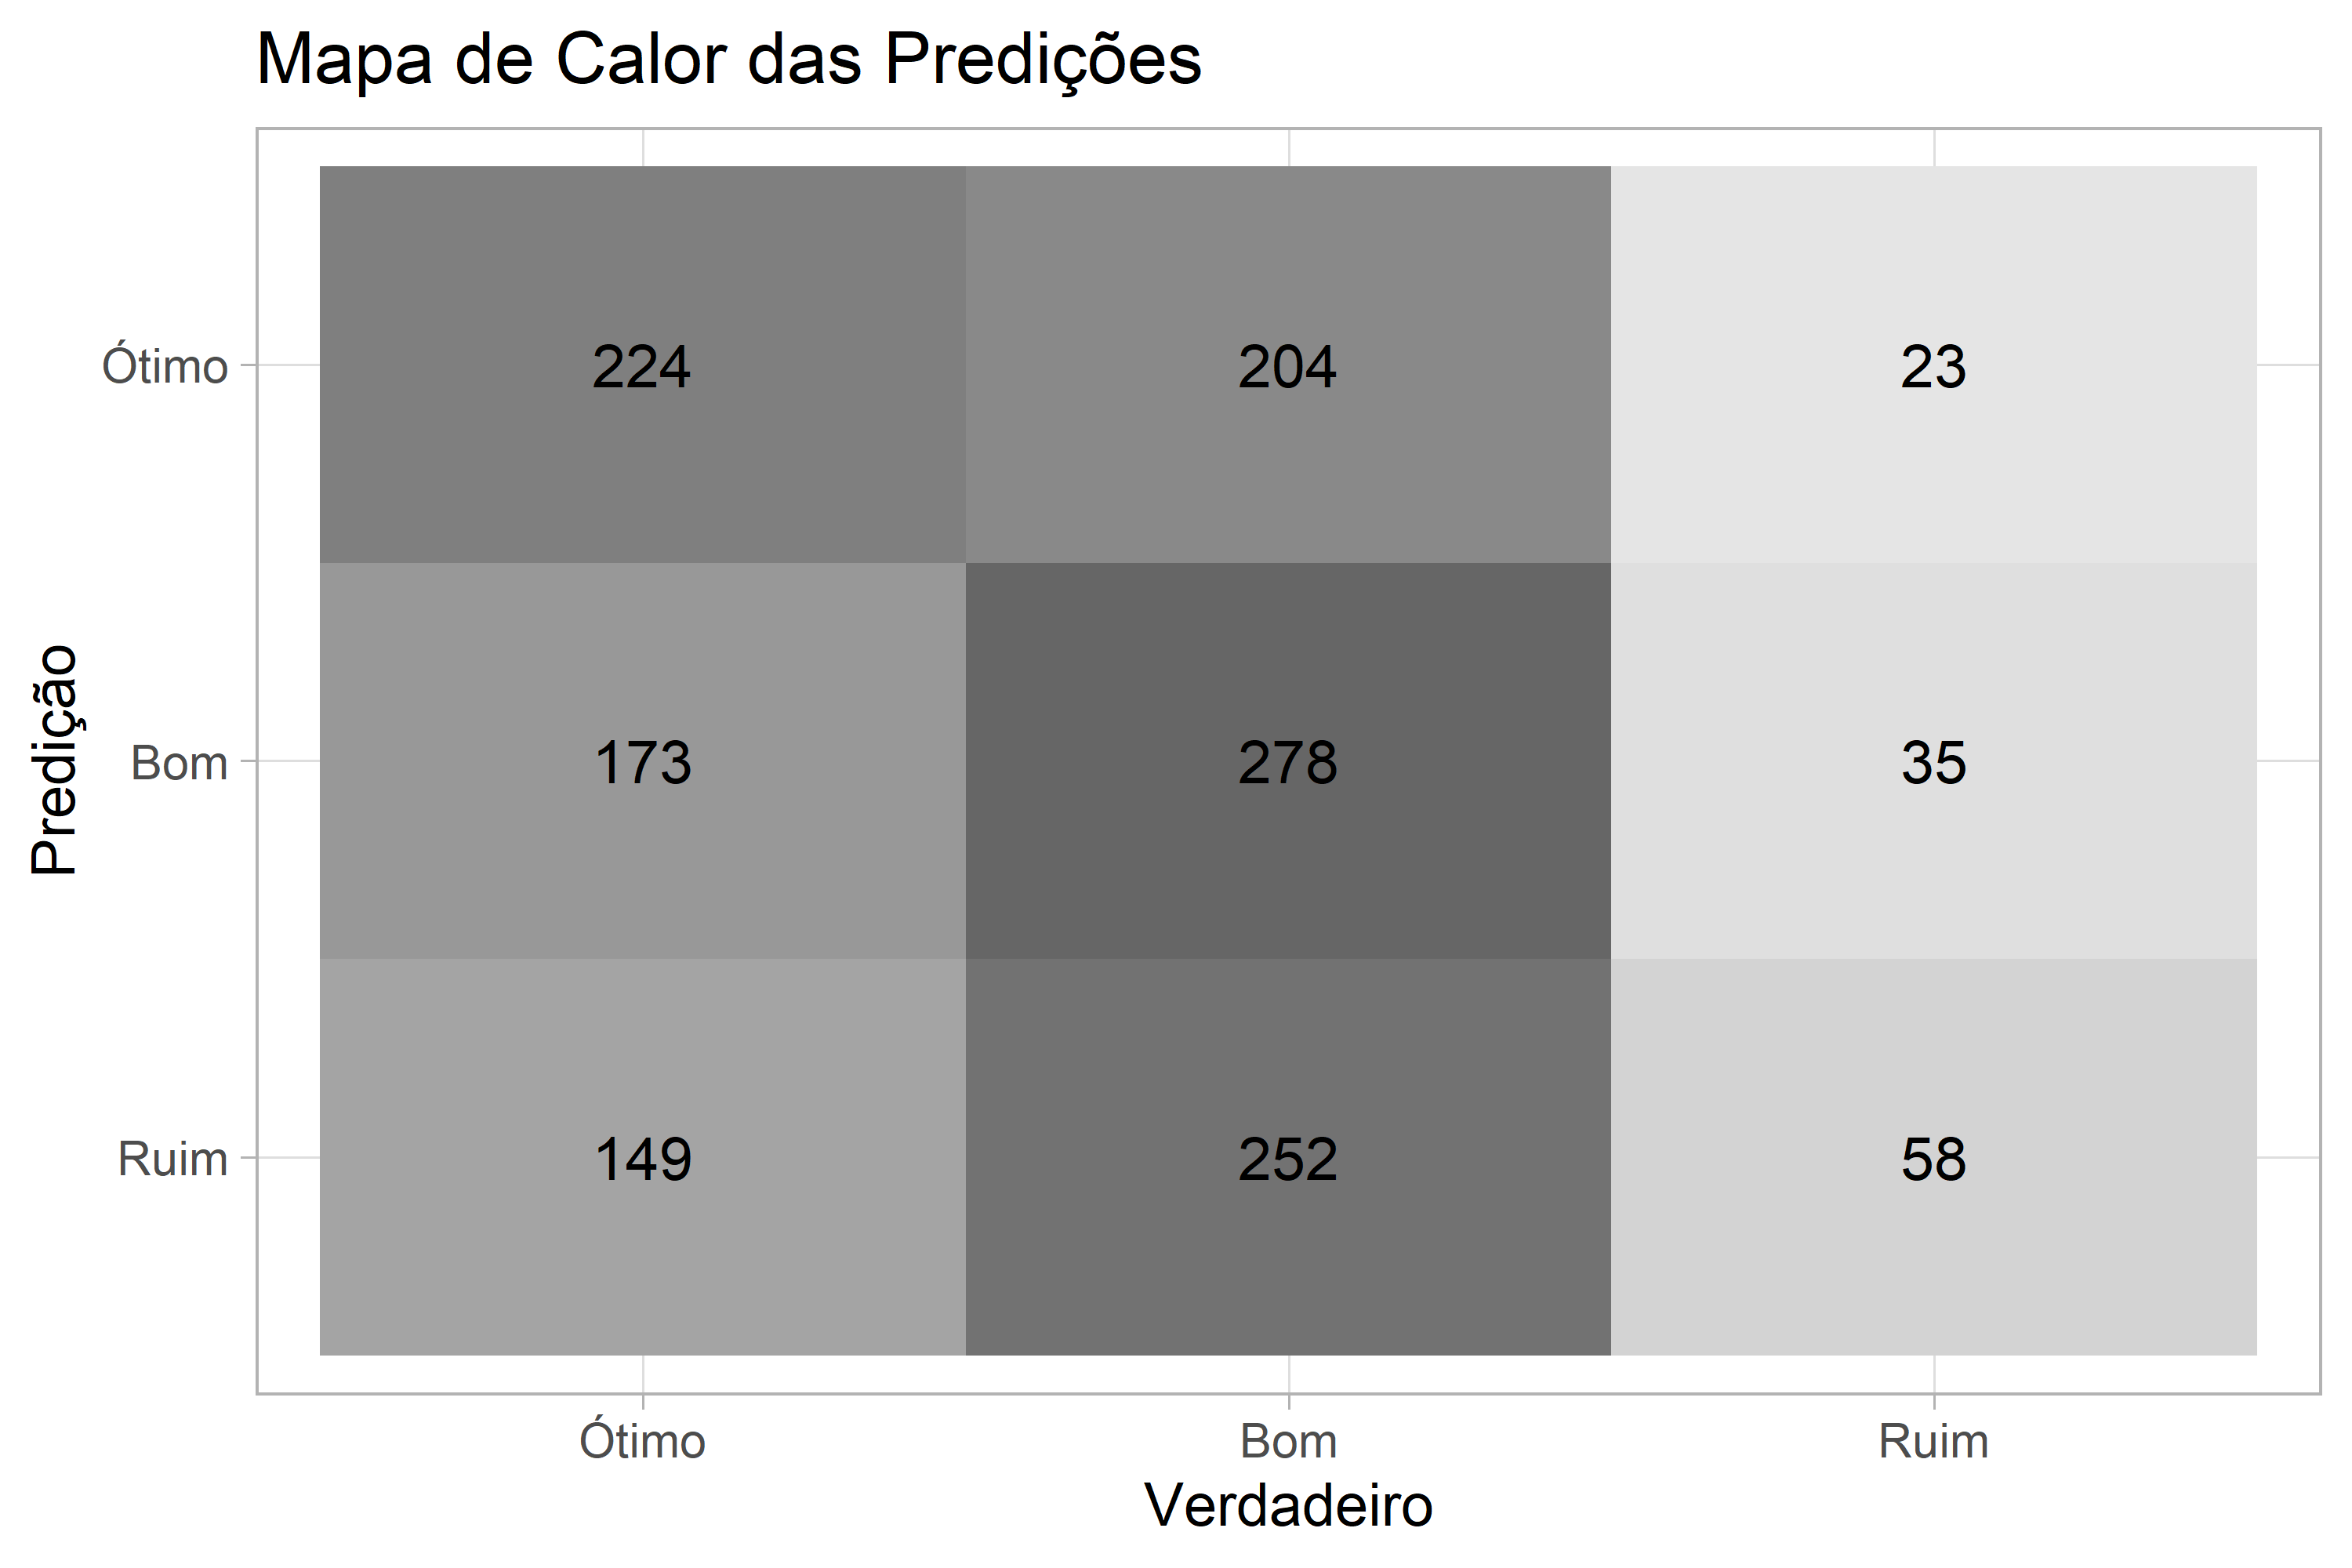
\includegraphics{apresentacao_files/figure-beamer/unnamed-chunk-23-1.png}
\end{frame}

\hypertarget{avaliando-a-curva-roc}{%
\subsubsection{Avaliando a Curva ROC}\label{avaliando-a-curva-roc}}

\begin{frame}{Avaliando a Curva ROC}
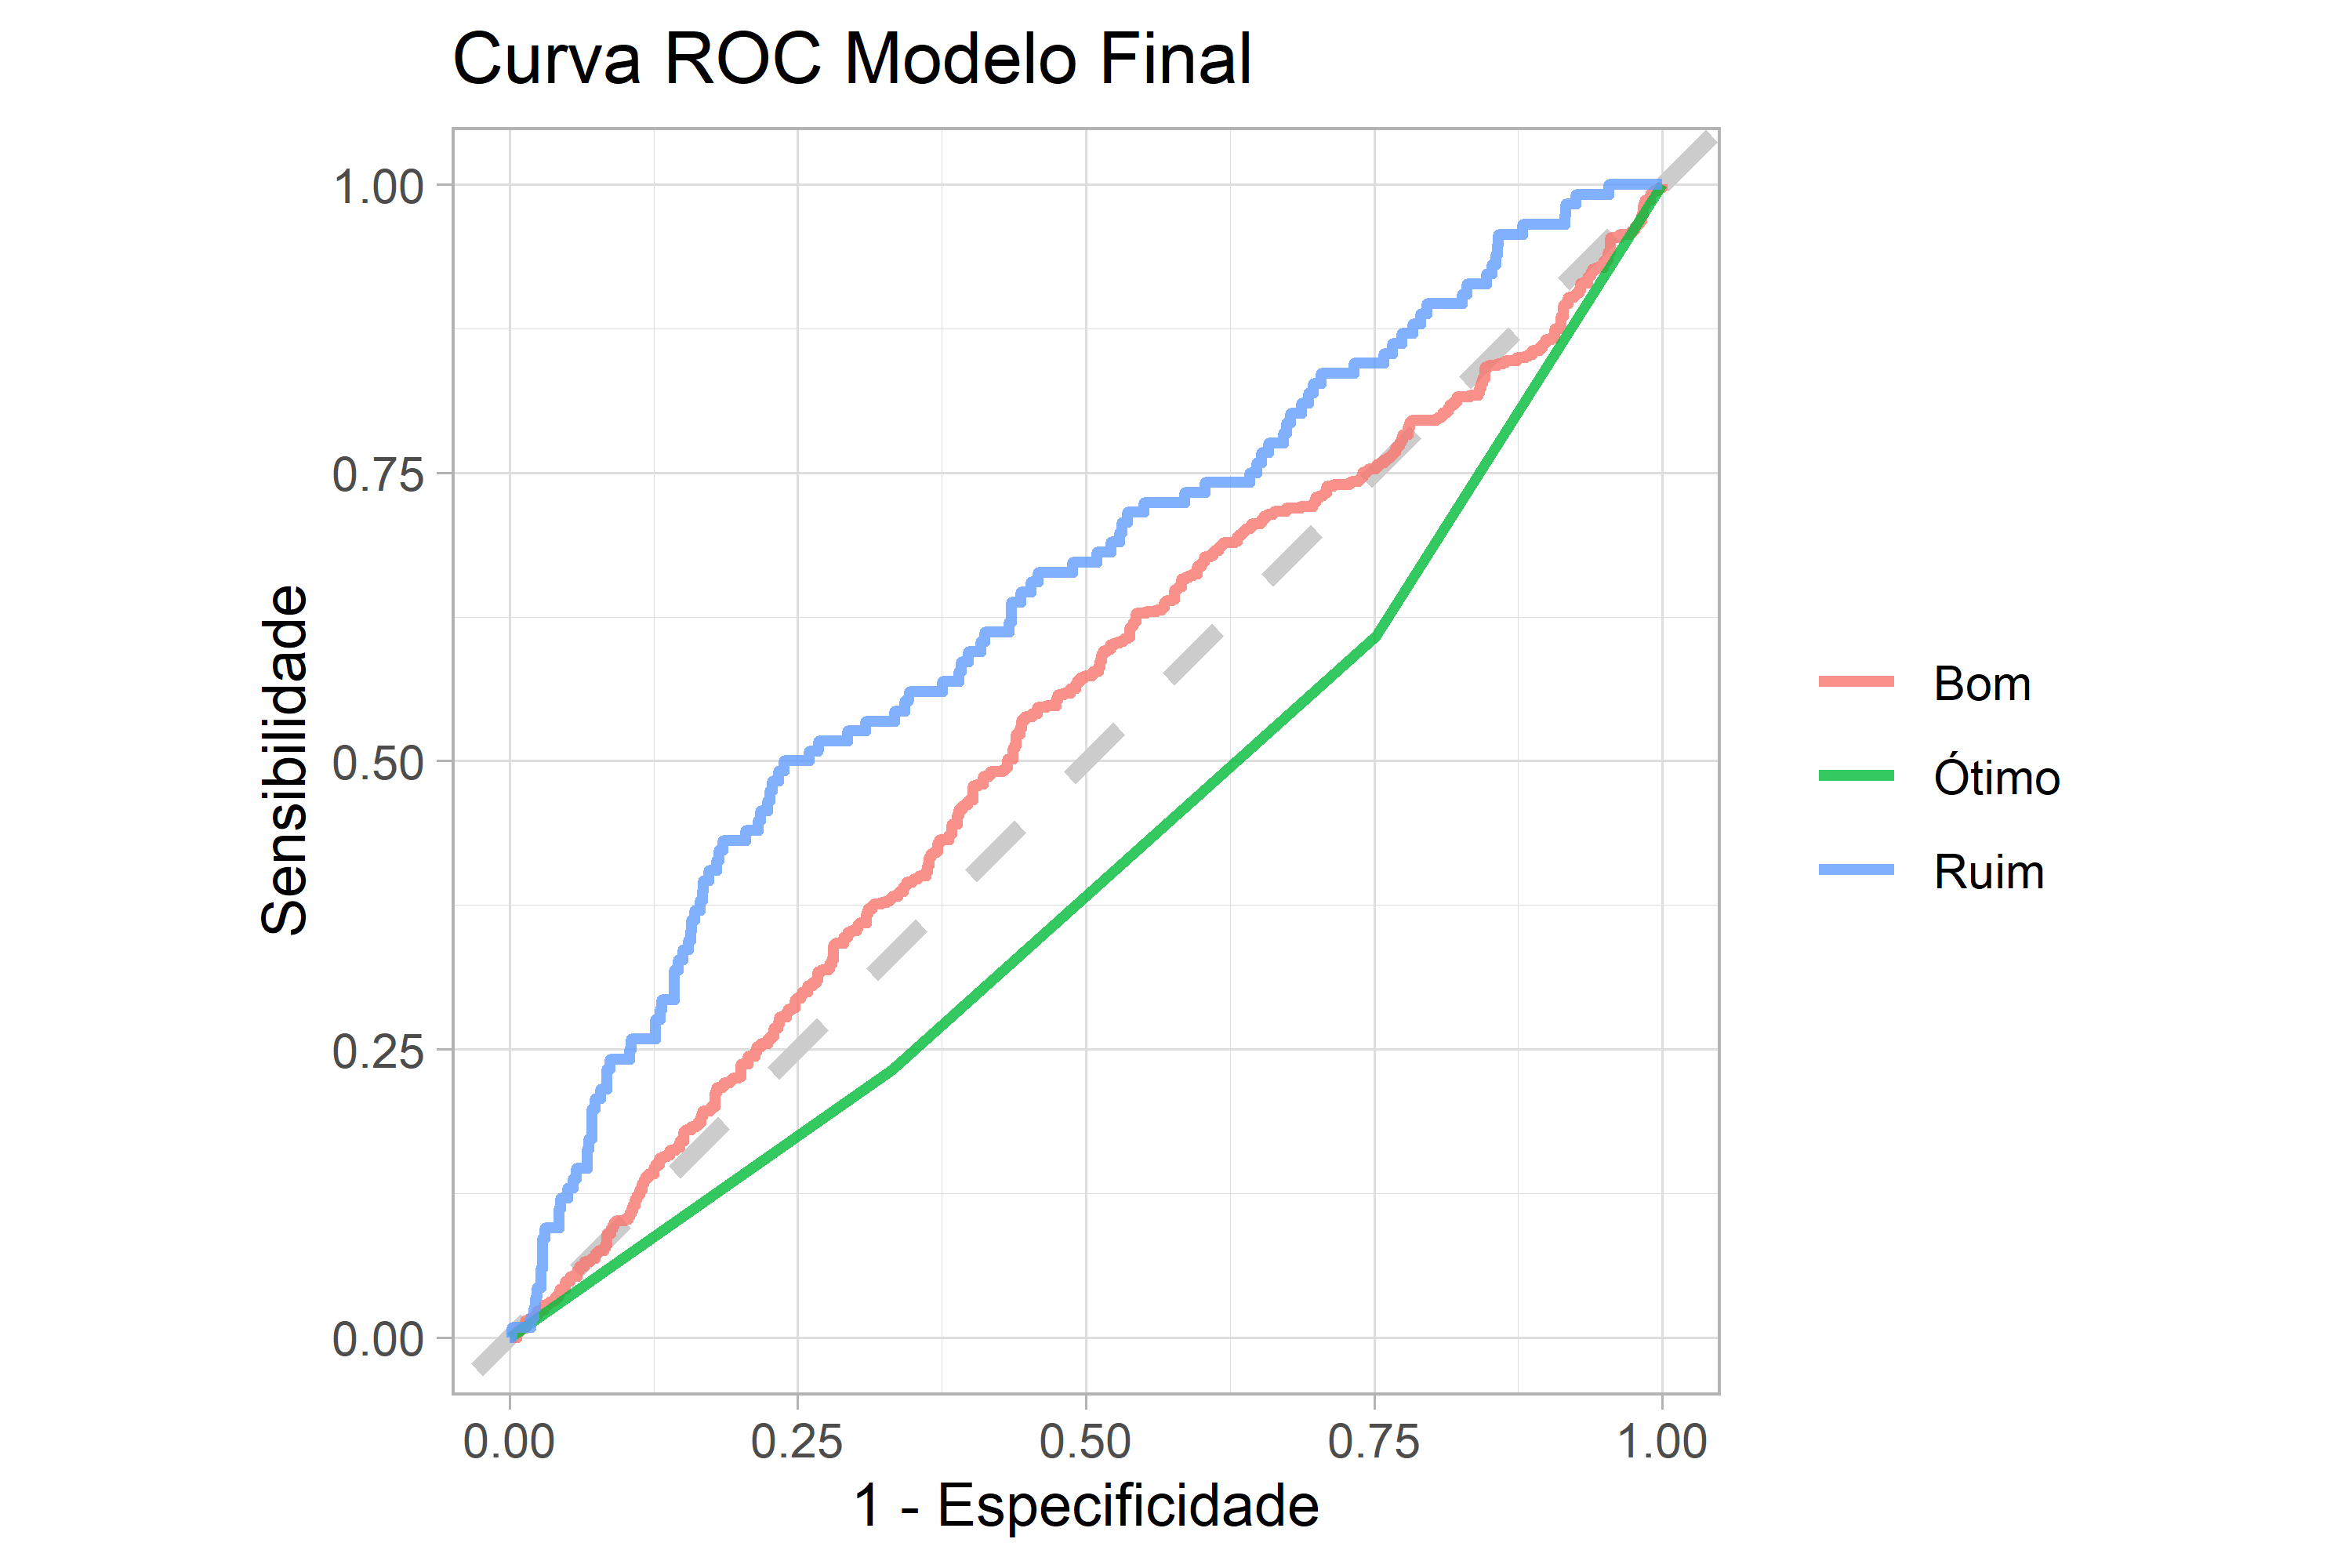
\includegraphics{apresentacao_files/figure-beamer/unnamed-chunk-24-1.png}
\end{frame}

\hypertarget{conclusuxe3o}{%
\section{Conclusão}\label{conclusuxe3o}}

\hypertarget{se-o-modelo-disser-que-o-livro-uxe9-uxf3timo-desconfie}{%
\subsubsection{Se o modelo disser que o livro é ÓTIMO,
desconfie\ldots{}}\label{se-o-modelo-disser-que-o-livro-uxe9-uxf3timo-desconfie}}

\begin{frame}{Se o modelo disser que o livro é ÓTIMO, desconfie\ldots{}}
\begin{itemize}
\tightlist
\item
  Algumas métricas:
\end{itemize}

\begin{table}[H]
\centering
\begin{tabular}{llr}
\toprule
.metric & .estimator & .estimate\\
\midrule
sens & macro & 0.4297\\
\bottomrule
\end{tabular}
\end{table}

\begin{table}[H]
\centering
\begin{tabular}{llr}
\toprule
.metric & .estimator & .estimate\\
\midrule
spec & macro & 0.7018\\
\bottomrule
\end{tabular}
\end{table}

\begin{table}[H]
\centering
\begin{tabular}{lrr}
\toprule
.level & mean\_sens & mean\_spec\\
\midrule
Bom & 0.5144 & 0.5152\\
Ótimo & 0.5725 & 0.3805\\
Ruim & 0.6383 & 0.5100\\
\bottomrule
\end{tabular}
\end{table}
\end{frame}

\hypertarget{mais-algumas-considerauxe7uxf5es}{%
\subsubsection{Mais algumas
considerações\ldots{}}\label{mais-algumas-considerauxe7uxf5es}}

\begin{frame}{Mais algumas considerações\ldots{}}
\begin{itemize}
\item
  A parte da engenharia de dados, como já comentada, além de desafiadora
  realiza importante papel na qualidade do modelo
\item
  Algumas mudanças poderiam melhorar o modelo, tais como:

  \begin{itemize}
  \tightlist
  \item
    uma melhora na limpeza dos dados, removendo ainda mais outliers;
  \item
    melhor definição nos níveis e categorias das variáveis preditoras;
  \item
    variáveis preditoras mais informativas e com mais distinção entre os
    níveis.
  \end{itemize}
\item
  Por fim, não consideramos satisfatório a capacidade preditora do
  modelo e concluímos que a melhor forma de saber se um livro é
  \emph{ótimo}, \emph{bom} ou \emph{ruim}, é lendo-o. ;)
\end{itemize}
\end{frame}

\hypertarget{referuxeancias}{%
\subsubsection{Referências:}\label{referuxeancias}}

\begin{frame}{Referências:}
\begin{itemize}
\item
  MORDE, Vishal. \textbf{XGBoost Algorithm: Long May She Reign!} -
  Abril, 2019. Publicado em \emph{Towards Data Science}. Disponível em:
  \url{https://towardsdatascience.com/https-medium-com-vishalmorde-xgboost-algorithm-long-she-may-rein-edd9f99be63d}
\item
  SILGE, Julia. \textbf{Tune xgboost models with early stopping to
  predict shelter animal status} - Agosto, 2021. Publicado em Julia
  Silge. Disponível em:
  \url{https://juliasilge.com/blog/shelter-animals/}
\item
  R Core Team (2021). \textbf{R:\emph{A language and environment for
  statistical computing}} . R Foundation for Statistical Computing,
  Vienna, Austria. URL \url{https://www.R-project.org/}.
\item
  SOUMIK . \textbf{Goodreads-books \emph{comprehensive list of books
  listed in goodreads}} - Maio, 2019. Publicado em Kagle. Disponível em:
  \url{https://www.kaggle.com/jealousleopard/goodreadsbooks}
\end{itemize}
\end{frame}

\end{document}
